% arara: xelatex: {shell: yes}
% arara: biber
% arara: xelatex: {shell: yes}
% arara: xelatex: {shell: yes}

% TODO: переформатировать разделы!
% TODO: задачки на тестирование гипотез с байесовским подходом до классического!
% TODO: это позволяет объяснить разницу между p-value и P(H_0|данные)
% TODO: как обозначить p-value? P(S_{\text{new}} > S \mid S, H_0)?

% Здесь мы держим компромисс между красотой и легкостью включения новых людей в процесс создания.
% Поэтому не используем пакеты, которые требуют возни с установкой и настройкой.
% Например, используем listings вместо minted.
% Пакет minted требует настроенного питона и связки латех-питон. 
% Вместо arara используем классический latexmk. 

%!TeX cleanPatterns = $OUTDIR/$JOB!($OUTEXT|.synctex.gz|.tex|.pdf), /$OUTDIR/_minted-$JOB/
\documentclass[12pt, a4paper]{article}

% utf8 is the preferred encoding

 % this magick is to solve problem that appeared after update of texlive 2018 to texlive 2020
 % https://tex.stackexchange.com/questions/511341/the-error-occurred-after-the-last-update
\makeatletter
\def\nobreak{\penalty\@M}
\makeatother


\usepackage{fontspec} % что-то про шрифты? % нужно ли загружать?

\usepackage{polyglossia} % русификация xelatex
\usepackage{csquotes}
\usepackage{wrapfig} % обтекание картинок



\setmainlanguage{russian}

% download "Linux Libertine" fonts:
% http://www.linuxlibertine.org/index.php?id=91&L=1
\setmainfont{Linux Libertine O} % or Helvetica, Arial, Cambria
% why do we need \newfontfamily:
% http://tex.stackexchange.com/questions/91507/
\newfontfamily{\cyrillicfonttt}{Linux Libertine O}

\newfontfamily\arabicfont[Script=Arabic]{Scheherazade New}


\usepackage{etoolbox} % provides \AtEndPreamble
% etoolbox causes wrong behavior of tocbasic
\AtEndPreamble{ % ради арабского написания Абу ибн-Сина
  \usepackage{arabxetex} 
 \let\textarabic\relax 
 \let\Arabic\relax 
\setotherlanguages{arabic, english}
}
% комбо из:
% https://tex.stackexchange.com/questions/501897
% https://tex.stackexchange.com/questions/392175/

\usepackage{imakeidx} 
\indexsetup{level=\section}
\makeindex[title=Модные хэштэги]

% \usepackage{etex} % расширение классического tex
% в частности позволяет подгружать гораздо больше пакетов, чем мы и займёмся далее
% message: extended allocation already in use

\usepackage{verbatim} % для многострочных комментариев
\usepackage{makeidx} % для создания предметных указателей

\usepackage{setspace}
\usepackage{amsmath, amsfonts, amssymb, amsthm}
\usepackage{mathrsfs} % sudo yum install texlive-rsfs
\usepackage{dsfont} % sudo yum install texlive-doublestroke
\usepackage{array, multicol, multirow, bigstrut} % sudo yum install texlive-multirow
\usepackage{indentfirst} % установка отступа в первом абзаце главы


\usepackage{bm}
\usepackage{bbm} % шрифт с двойными буквами
%\usepackage[perpage]{footmisc}

\usepackage{dcolumn} % центрирование по разделителю для apsrtable

% создание гиперссылок в pdf
\usepackage[unicode, colorlinks=true, urlcolor=blue, hyperindex, breaklinks]{hyperref}


\usepackage{microtype} % свешиваем пунктуацию
% теперь знаки пунктуации могут вылезать за правую границу текста, при этом текст выглядит ровнее


\usepackage{textcomp}  % Чтобы в формулах можно было русские буквы писать через \text{}

% размер листа бумаги
%\usepackage[paperwidth=145mm,paperheight=215mm,
%height=182mm,width=113mm,top=20mm,includefoot]%{geometry}
\usepackage[paper=a4paper, top=15mm, bottom=13.5mm, left=16.5mm, right=13.5mm, includefoot]{geometry}

\usepackage{xcolor}
\usepackage{framed} % для рамок и черты слева от минитеории, \leftbar


% \usepackage{float, longtable}
% \usepackage{soulutf8}

\usepackage{enumitem} % дополнительные плюшки для списков
%  например \begin{enumerate}[resume] позволяет продолжить нумерацию в новом списке

\usepackage{mathtools}
\usepackage{cancel, xspace} % sudo yum install texlive-cancel


\usepackage{numprint} % sudo yum install texlive-numprint
\npthousandsep{,}\npthousandthpartsep{}\npdecimalsign{.}


% \usepackage{subfigure} % для создания нескольких рисунков внутри одного

\usepackage{tikz, pgfplots} % язык для рисования графики из latex'a
\pgfplotsset{compat=1.16}
\usetikzlibrary{trees} % tikz-прибамбас для рисовки деревьев
\usepackage{tikz-qtree} % альтернативный tikz-прибамбас для рисовки деревьев
\usetikzlibrary{arrows} % tikz-прибамбас для рисовки стрелочек подлиннее

\usepackage{todonotes} % для вставки в документ заметок о том, что осталось сделать
% \todo{Здесь надо коэффициенты исправить}
% \missingfigure{Здесь будет Последний день Помпеи}
% \listoftodos — печатает все поставленные \todo'шки



\usepackage{booktabs} %  красивые таблицы
% заповеди из докупентации:
% 1. Не используйте вертикальные линни
% 2. Не используйте двойные линии
% 3. Единицы измерения - в шапку таблицы
% 4. Не сокращайте .1 вместо 0.1
% 5. Повторяющееся значение повторяйте, а не говорите "то же"

\usepackage{physics}

\usepackage{listings}
\lstset{%
basicstyle=\fontfamily{lmtt}\bfseries,
keywordstyle=\fontfamily{lmtt}\bfseries
}
\usepackage{answers}




\usepackage[bibencoding=auto, backend=biber, sorting=none, style=alphabetic]{biblatex}

\addbibresource{probability_pro.bib}

\setcounter{tocdepth}{1} % в оглавление оставляем уровень 1

\usepackage[titles]{tocloft} % альтернатива tocbasic для настройки toc
% если нужен subfigure, то у tocloft можно добавить опцию subfigure
\renewcommand{\cftbeforesecskip}{0.7pt} % поправка интервала между строками для section в toc
\renewcommand{\cftsecdotsep}{\cftdotsep} % добавляем точечки

\AddEnumerateCounter{\asbuk}{\russian@alph}{щ} % для списков с русскими буквами
\setlist[enumerate, 1]{label=\asbuk*),ref=\asbuk*} % цифра рядом с enumerate = уровень нумерации



%%%%%%%%%%%%%%%%%%%%%%%  ПАРАМЕТРЫ  %%%%%%%%%%%%%%%%%%%%%%%%%%%%%%%%%%
\setstretch{1}                          % Межстрочный интервал
\flushbottom                            % Эта команда заставляет LaTeX чуть растягивать строки, чтобы получить идеально прямоугольную страницу
\righthyphenmin=2                       % Разрешение переноса двух и более символов
%\pagestyle{plain}                       % Нумерация страниц снизу по центру.
\widowpenalty=300                     % Небольшое наказание за вдовствующую строку (одна строка абзаца на этой странице, остальное — на следующей)
\clubpenalty=3000                     % Приличное наказание за сиротствующую строку (омерзительно висящая одинокая строка в начале страницы)
\setlength{\parindent}{1.5em}           % Красная строка.
%\captiondelim{. }
\setlength{\topsep}{0pt}
\emergencystretch=2em

% делаем короче интервал в списках
\setlength{\itemsep}{0pt}
\setlength{\parskip}{0pt}
\setlength{\parsep}{0pt}



\DeclareMathOperator{\card}{card}
\DeclareMathOperator{\sign}{sign}
\DeclareMathOperator{\sgn}{sign}
\DeclareMathOperator{\Span}{span} 
% we can't use \span because it's used by multicol and amsmath
% https://tex.stackexchange.com/questions/33264/span-as-a-math-operator

\DeclareMathOperator*{\argmin}{arg\,min}
\DeclareMathOperator*{\amn}{arg\,min}
\DeclareMathOperator*{\amx}{arg\,max}


\DeclareMathOperator{\Corr}{Corr}
\DeclareMathOperator{\sCorr}{sCorr}
\DeclareMathOperator{\sCov}{sCov}
\DeclareMathOperator{\sVar}{sVar}

\DeclareMathOperator{\Cov}{Cov}
\DeclareMathOperator{\Var}{Var}
\DeclareMathOperator{\cov}{Cov}
\DeclareMathOperator{\Bin}{Bin}
\DeclareMathOperator*{\plim}{plim}
\DeclareMathOperator{\MSE}{MSE}
\DeclareMathOperator{\softmax}{softmax}
\DeclareMathOperator{\Med}{Med}


\renewcommand{\P}{\mathbb{P}}
\newcommand{\E}{\mathbb{E}}

\newcommand{\e}{\varepsilon}

\newcommand{\cN}{\mathcal{N}}
\newcommand{\dNorm}{\mathcal{N}}
\newcommand{\dN}{\mathcal{N}}
\newcommand{\dLN}{\mathcal{LN}}

\newcommand{\dBern}{\mathrm{Bern}}
\newcommand{\dPois}{\mathrm{Pois}}
\newcommand{\dBin}{\mathrm{Bin}}
\newcommand{\dMult}{\mathrm{Mult}}
\newcommand{\dGeom}{\mathrm{Geom}}
\newcommand{\dNHGeom}{\mathrm{NHGeom}}
\newcommand{\dHGeom}{\mathrm{HGeom}}
\newcommand{\dDUnif}{\mathrm{DUnif}}
\newcommand{\dFS}{\mathrm{FS}}
\newcommand{\dNBin}{\mathrm{NBin}}

\newcommand{\dTri}{\mathrm{Triangle}}
\newcommand{\dUnif}{\mathrm{Unif}}
\newcommand{\dCauchy}{\mathrm{Cauchy}}
\newcommand{\dExpo}{\mathrm{Expo}}
\newcommand{\dBeta}{\mathrm{Beta}}
\newcommand{\dGamma}{\mathrm{Gamma}}
\newcommand{\dWei}{\mathrm{Wei}}
\newcommand{\dLogistic}{\mathrm{Logistic}}
\newcommand{\dRayleigh}{\mathrm{Rayleigh}}
\newcommand{\dPareto}{\mathrm{Pareto}}


% вместо горизонтальной делаем косую черточку в нестрогих неравенствах
\renewcommand{\le}{\leqslant}
\renewcommand{\ge}{\geqslant}
\renewcommand{\leq}{\leqslant}
\renewcommand{\geq}{\geqslant}


\newcommand{\wv}{\textrm{word2vec}}
\newcommand \hVar{\widehat{\Var}}
\newcommand \hCorr{\widehat{\Corr}}
\newcommand \hCov{\widehat{\Cov}}


\newcommand{\RR}{\mathbb{R}}


\title{Заметки к семинарам по статистике}
\author{\url{https://github.com/bdemeshev/statistics_pro}}
\date{\today}


%\newtheorem{problem}{Задача}
%\numberwithin{problem}{section}

\Newassociation{sol}{solution}{solution_file}
% sol — имя окружения внутри задач
% solution — имя окружения внутри solution_file
% solution_file — имя файла в который будет идти запись решений
% можно изменить далее по ходу
\Opensolutionfile{solution_file}[all_solutions]
% в квадратных скобках фактическое имя файла



% магия для автоматических гиперссылок задача-решение
\newlist{myenum}{enumerate}{3}
% \newcounter{problem}[chapter] % нумерация задач внутри глав
\newcounter{problem}[section]

\newenvironment{problem}%
{%
\refstepcounter{problem}%
%  hyperlink to solution
     \hypertarget{problem:{\thesection.\theproblem}}{} % нумерация внутри глав
     % \hypertarget{problem:{\theproblem}}{}
     \Writetofile{solution_file}{\protect\hypertarget{soln:\thesection.\theproblem}{}}
     %\Writetofile{solution_file}{\protect\hypertarget{soln:\theproblem}{}}
     \begin{myenum}[label=\bfseries\protect\hyperlink{soln:\thesection.\theproblem}{\thesection.\theproblem},ref=\thesection.\theproblem]
     % \begin{myenum}[label=\bfseries\protect\hyperlink{soln:\theproblem}{\theproblem},ref=\theproblem]
     \item%
    }%
    {%
    \end{myenum}}
% для гиперссылок обратно надо переопределять окружение
% это происходит непосредственно перед подключением файла с решениями


\newcommand{\addtag}[1]{\index{#1}}




\begin{document}

\maketitle % ставим сюда название, автора и время создания

% здесь нужна прикольная картинка

\newpage
\tableofcontents{}

\newpage

Это задачки по статистике. 
При везении подсказку, ответ или решение можно найти, кликнув по номеру задачи. 
Свежая версия доступна по ссылке \url{https://github.com/bdemeshev/statistics_pro}.
Красивые и сложные олимпиадные задачи по вероятностям можно найти по ссылке \url{https://github.com/bdemeshev/probability_dna},
подборку прошлых экзаменов вшэ — \url{https://github.com/bdemeshev/probability_hse_exams},
а задачки к семинарам по вероятностями — \url{https://github.com/bdemeshev/probability_pro}.

Если \url{github.com} не доступен, то можно попробовать зеркало на \url{gitlab.com}.

\section{Статистика ноль}

\begin{leftbar}
Среднее, $\bar x = (x_1 + \ldots + x_n) / n$. 
Медиану в случае непрерывной функции распределения находим из условия $\P(X \geq \Med X) = 0.5$, $\P(X \leq \Med X) = 0.5$.
Медиану в общем случае находим из условия $\P(X \geq \Med X) \geq 0.5$, $\P(X \leq \Med X) \geq 0.5$.
\end{leftbar}

\begin{problem}
  Имеется пять действительных чисел: $x$, $9$, $5$, $4$, $7$. При каком значении $x$ медиана будет равна среднему?


\begin{sol}
Среднее равно $(x+25)/5$. Если $x<5$, получаем $x=0$. Если $x \in (5; 7)$, получаем $x=25/4$. Если $x>7$, получаем $x=10$.
\end{sol}
\end{problem}

\begin{problem}
Измерен рост 25 человек. Средний рост оказался равным 160 см. 
Медиана оказалась равной 155 см. 
Машин рост в 163 см был ошибочно внесен как 173 см. 

\begin{enumerate}
  \item Как изменятся медиана и среднее после исправления ошибки?
  \item А как могут измениться медиана и среднее, если истинный рост Маши равен 153?
\end{enumerate}

\begin{sol}
Медиана не изменится, среднее упадёт на $10/25=0.4$. 
Для случая роста $153$: среднее упадёт на $0.8$, медиана упадёт произвольно на некое число из отрезка $[0;2]$.
\end{sol}

\end{problem}
\begin{problem}
Возможно ли чисто теоретически, что риск катастрофы в расчете на 1 час пути
больше для самолета, чем для автомобиля, 
а в расчете на 1 километр пути — наоборот?

\begin{sol}
  да
\end{sol}
\end{problem}

\begin{problem}
Деканат утверждает, что если Вовочку перевести из группы
А в группу В, то средний рейтинг каждой группы возрастет. 

Возможно ли это?
\begin{sol}
да
\end{sol}
\end{problem}

\begin{problem}
Есть три группы по 10 человек, две группы по 20 человек и одна группа из 40 человек. 
У каждой из групп свой преподаватель.
\begin{enumerate}
\item Каков средний размер группы, для которой читает лекции наугад выбранный профессор?
\item Каков средний размер группы, в которой учится наугад выбранный студент?
\item Творческий вопрос. 
Мы ловим студентов наугад и спрашиваем каждого размер группы, в которой он учится. 
Можно ли как-то восстановить средний размер группы с точки зрения преподавателя?
\end{enumerate}


\begin{sol}
\end{sol}
\end{problem}



\begin{problem}
Приведите примеры случайных величин $X$ и $Y$, для которых:
\begin{enumerate}
\item $\Med(X+Y)=\Med(X)+ \Med(Y)$;
\item $\Med(X+Y) \neq \Med(X)+ \Med(Y)$;
\item $\Med(X^k)=\Med(X)^k$ для всех $k$;
\item $\Med(X^2)\neq \Med(X)^2$.
\end{enumerate}

\begin{sol}
  \begin{enumerate}
    \item Для $\Med(X+Y)=\Med(X)+ \Med(Y)$ можно взять два независимых симметричных распределения.
    \item Для $\Med(X+Y) \neq \Med(X)+ \Med(Y)$ подойдёт практически любая сумма несимметричных распределений.
    Например, можно взять две независимых величины с плотностью $f(x)=2-2x$ на отрезке $[0;1]$.
    \item Для $\Med(X^k)=\Med(X)^k$ для всех $k$ можно взять неотрицательную случайную величину.
    \item Для $\Med(X^2)\neq \Med(X)^2$ подойдёт симметричная около нуля случайная величина.
    \end{enumerate}
    
\end{sol}
\end{problem}



\begin{problem}
Исследователь Вениамин измерил рост пяти случайно выбранных человек. 
Рост имеет непрерывное распределение.
 
Какова вероятность того, что истинная медиана роста лежит между минимумом и максимумом из этих пяти наблюдений? 
\begin{sol}
  Исключим те варианты, когда все пять наблюдений оказались или синхронно выше, или синхронно ниже медианы, получаем, $p=1-2\cdot 0.5^5=1-0.5^4$.
\end{sol}
\end{problem}


\begin{problem}
 Во время Второй Мировой войны американские военные собрали статистику попаданий пуль в фюзеляж самолёта.  
 По самолётам, вернувшимся из полёта на базу, была составлена карта повреждений среднестатистического самолёта. 
 С этими данными военные обратились к статистику Абрахаму Вальду с вопросом, в каких местах следует увеличить броню самолёта.

Что посоветовал Абрахам Вальд и почему?

\begin{sol}
Укреплять те места, где не было следов пуль.
\end{sol}
\end{problem}



\begin{problem}
 Два лекарства испытывали на мужчинах и женщинах. 
 Каждый человек принимал только одно лекарство. 
 Общий процент людей, почувствовавших улучшение, больше среди принимавших лекарство А.
Процент мужчин, почувствовавших улучшение, больше среди мужчин, принимавших лекарство В. 
Процент женщин, почувствовавших улучшение, больше среди женщин, принимавших лекарство В.

\begin{enumerate}
\item Возможно ли это?
\item Какое лекарству нужно порекомендовать больному, не зная его пола?
\end{enumerate}

\begin{sol}
\end{sol}
\end{problem}


\begin{problem}
 Из набора чисел $\{2,4,10,14\}$ случайным образом равновероятно по очереди выбираются три числа с возможностью повторения.

\begin{enumerate}
\item Найдите закон распеределения (табличку с вероятностями) величины $X_1$. Найдите закон распределения величины $X_2$.
\item Найдите совместный закон распределения пары $X_1$, $X_2$. Найдите совместный закон распределения пары $X_1$, $X_3$.
\item Являются величины $X_1$, $X_2$, $X_3$ независимыми? Одинаково распределеннными?
\item Верно ли, что $\E(X_1)=\E(X_2)=\E(X_3)$? Верно ли, что $\Var(X_1)=\Var(X_2)=\Var(X_3)$?
\item Верно ли, что $\Cov(X_1,X_2)=\Cov(X_1,X_3)$?
\item Как изменятся ответы на предыдущие вопросы, если числа выбираются без возможности повторения?
\end{enumerate}


\begin{sol}
\end{sol}
\end{problem}




\begin{problem}
 Из фиксированного множества $N$ чисел случайным образом выбирают $n$ чисел. Известно, что если бы выбирать наугад всего одно число, то тогда математическое ожидание и дисперсие этого одного случайного числа были бы равны $\E(X_1)=\mu$ и $\Var(X_1)=\sigma^2$. Обозначим среднее арифметическое выбранных $n$ чисел с помощью $\bar{X}_n$. Чему равны $\E(\bar{X}_n)$ и $\Var(\bar{X}_n)$, если:

\begin{enumerate}
\item Мы выбираем $n$ чисел из $N$ с возвращениями
\item Мы выбираем $n$ чисел из $N$ без возвращений
\item Во что превращаются полученные формулы при $n=1$? при $n=N$? при $N\to \infty$?
\end{enumerate}

\begin{sol}
\begin{enumerate}
\item $\E(\bar{X}_n) = \mu$, $\Var(\bar{X}_n) = \frac{\sigma^2}{n}$
\item $\E(\bar{X}_n) = \mu$, $\Var(\bar{X}_n) = \frac{\sigma^2}{n} \cdot \frac{N-n}{N-1}$
\item При $N\to \infty$ получится формула для выборки с возвращениями.
\end{enumerate}
\end{sol}
\end{problem}




\begin{problem}
 Исследовательница Мишель подбрасывает кубик\index{кубик} $100$ раз.
 Обозначим с помощью $X_i$ количество выпадений числа $i$ на всех кубиках. 
 Например, величина $X_1$ — это количество выпадений единицы, 
 а $X_6$ — количество выпадений шестёрки.
\begin{enumerate}
\item Как распределена величина $X_1$? Величина $X_6$? 
Найдите $\E(X_1)$, $\Var(X_1)$.
\item Верно ли, что величины $X_1$ и $X_6$ независимы? Одинаково распередены?
\item Найдите $\Cov(X_1, X_1+X_2+X_3+X_4+X_5+X_6)$, $\Cov(X_1,X_6)$.
\item Найдите $\Corr(X_1,X_6)$, проинтерпретируйте значение корреляции.
\end{enumerate}

\begin{sol}
\end{sol}
\end{problem}




\begin{problem}
 В множестве $A$ всего два числ, $A=\{24, 42\}$. Случайным образом из множества $A$ выбираются 3 числа с возможностью повторений. Явно найдите закон распределения выборочного среднего, выборочной медианы, выборочной моды, выборочного минимима и выборочного максимума.

\begin{sol}
\end{sol}
\end{problem}



\begin{problem}
  Величины $X$ и $Y$ независимы и одинаково распределены на отрезке $[0;1]$ с функцией плотности $f(x)=2x$.

  \begin{enumerate}
    \item Найдите теоретическую медиану $\Med(X)$.
    \item Найдите теоретическую медиану $\Med(X+Y)$.
  \end{enumerate}


  \begin{sol}
  $m^2=1/2$, $\Med(X) = 1/\sqrt{2}$.
\end{sol}
\end{problem}


\begin{problem}
Величины $X_1$, \ldots, $X_n$ — независимы и равномерны на отрезке $[0;1]$.
Узнав значения этих величин, исследовательница Кассандра случайно равновероятно с возможностью повторений выбирает 
из них значения $X_1^*$, \ldots, $X_n^*$. То есть, $X_1^*$ равновероятно равно $X_1$, $X_2$, \ldots, $X_n$. Аналогично, 
$X_2^*$ равновероятно равно $X_1$, $X_2$, \ldots, $X_n$. И так далее.

\begin{enumerate}
  \item Найдите $\E(\bar X)$, $\Var(\bar X)$;
  \item Найдите $\E(X_i^*)$, $\Var(X_i^*)$, $\Cov(X_i, X_j^*)$;
  \item Найдите $\E(\bar X^*)$, $\Var(\bar X^*)$, $\Cov(\bar X, \bar X^*)$;
\end{enumerate}

\begin{sol}
  $\E(X_i^*)=\E(X_i)$, $\Var(X_i^*)=\Var(X_i)$
\end{sol}
\end{problem}
 

\begin{problem}
  Аня, Боря и Вова поделили между собой натуральные числа от 1 до 27, включительно. 
  У Ани среднее выборочное равно 15, у Бори — 3, у Вовы — 18.

  Сколько чисел могло оказаться у Ани?

\begin{sol}
  
\end{sol}
\end{problem}


\section{Случайная выборка}


\begin{problem}
 Создайте случайную выборку объемом $n=1000$ из равномерного на отрезке $[0;1]$ распределения.
\begin{enumerate}
\item Найдите выборочные характеристики: среднее, медиану, минимум и максимум, стандартную ошибку, 10\%-ый и 95\%-ый квантили.
\item Постройте гистограмму распределения, выборочную функцию распределения для первых 20 чисел из случайной выборки
\item Повторите данный опыт для нормального $\cN(5,1)$ распределения и для экспоненциального  распределения с параметром $\lambda=1$
\item Насколько сильно выборочные характеристики отличаются от истинных?
\end{enumerate}

\begin{sol}
\end{sol}
\end{problem}

\begin{problem}
 Придумайте способ, как сгенерировать $100$ одинаково распределенных случайных величин, таких что $\sum_{i=1}^{100} X_i = 50$. 
 
 Будут ли эти величины $X_i$ зависимы?
 
 Модифицируйте способ, так чтобы он давал одинаково распределенные величины, такие что $\sum_{i=1}^{100} Y_i^2 = 50$. 
 Будут ли эти новые величины $Y_i$ зависимы?

\begin{sol}
\end{sol}
\end{problem}

\begin{problem}
 Придумайте детерминистическую функцию, такую, которая бы превращала одну равномерную на $[0;1]$ случайную величину $X$ в

\begin{enumerate}
\item случайную величину $Y$, принимающую значения $1$ и $0$ с вероятностями $0.7$ и $0.3$ соответственно
\item случайную величину $Z$ с функцией плотности $f(z)=2z$ на отрезке $z\in [0;1]$
\item пару независимых одинаково распределенных случайных величин $(Y_1, Y_2)$, принимающих значения $1$ и $0$ с вероятностями $0.7$ и $0.3$ соответственно
\item пару независимых равномерных на $[0;1]$ случайных величин
\end{enumerate}


\begin{sol}
\end{sol}
\end{problem}
\begin{problem}
 Постройте случайную выборку в $n=200$ наблюдений из двумерного нормального распределения с параметрами:

\begin{equation}
\begin{pmatrix}	X \\ 	Y 	\end{pmatrix}
\sim \cN
\left(
\begin{pmatrix}
25 \\ 125
\end{pmatrix}
;
\begin{pmatrix}
 5 & 4 \\
 4 & 10
 \end{pmatrix}
\right)
\end{equation}

\begin{enumerate}
\item Посчитайте выборочную ковариацию, выборочную корреляцию
\item Постройте диаграмму рассеяния, нанесите на диаграмму рассеяния линию $y(x)=E(Y|X=x)$
\item Насколько сильно выборочные характеристики отличаются от истинных?
\end{enumerate}

\begin{sol}
\end{sol}
\end{problem}
\begin{problem}
 Создайте $500$ выборок объемом $n=20$ каждая из равномерного на отрезке $[0;1]$ распределения и вычислите выборочное среднее для каждой из выборок.
\begin{enumerate}
\item Каково теоретическое математическое ожидание и дисперсия каждого из выборочных средних?
\item Постройте гистограмму выборочных средних
\item На фоне функции плотности стандартного нормального распределения изобразите в подходящем масштабе гистограмму стандартизированных выборочных средних
\end{enumerate}

\begin{sol}
\end{sol}
\end{problem}

\section{Проецируй!}

\begin{leftbar}
Если
\begin{enumerate}
  \item вектор $Z$ имеет многомерное нормальное стандартное распределение, $Z\sim \cN(0; I)$,
  \item $\hat Z$ — это проекция вектора $Z$ на некоторое $d$-мерное подпространство $V$,
  \item $Q$ — это квадрат длины проекции, $Q=||\hat Z||^2$,
\end{enumerate}
то закон распределения величины $Q$ называется  \textit{хи-квадрат распределением} с $d$ степенями свободы и обозначается $Q \sim \chi^2_d$.
\end{leftbar}

\begin{problem}
  Вектор $Z$ имеет многомерное нормальное распределение, $Z_i \sim \cN(0;1)$, и все $Z_i$ независимы.
  Для каждого случая найдите проекцию $\hat Z$ вектора $Z$ на подпространство $V$;
  найдите квадрат длины проекции, $Q$; укажите закон распределения величины $Q$:
  \begin{enumerate}
    \item $V = \Span(e)$, где $e=(1, 1, 1, 1, \ldots, 1)$;
    \item $V = \Span(e)$, где $e=(1, 2, 3, 4, \ldots, n)$;
    \item $V = \Span(e_1, e_2)$, где $e_1=(1, 0, 0, 0, \ldots, 0)$, $e_2 = (0, 1, 1, 1, \ldots, 1)$;
    \item $V = (\Span(e))^{\perp}$, где $e=(1, 1, 1, 1, \ldots, 1)$;
    \item $V = \Span(e_5, e_7, e_9)$, вектор $e_i$ содержит $1$ на $i$-ом месте и $0$ на остальных;
  \end{enumerate}

\begin{sol}
Здесь потребуется формула для $S=1^2+2^2 + \ldots + n^2$.

На рисунке сложены три суммы:

\begin{minipage}{0.8\textwidth}
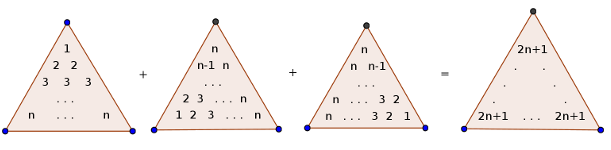
\includegraphics[width=\textwidth]{figure/triangle-proof.png}
\end{minipage}

На языке формул:
\[
  3S = (2n+1) \cdot (1 + 2 + \ldots + n) = (2n+1)n\frac{n+1}{2}.
\]
\end{sol}
\end{problem}




\begin{problem}
  Найдите минимум функции $f(a, b, c) = (6-a)^2 + (3 - b)^2 + (7 - b)^2 + (8 - c)^2 + (9-c)^2 + (10- c)^2 + 11^2$;

  Проекцией какого вектора на какое пространство является вектор $\hat Z = (a^*, b^*, b^*, c^*, c^*, c^*, 0)$?
\begin{sol}
  Минимум, $a=6$, $b=5$, $c= 9$.
  Например, проекцией вектора $(6, 3, 7, 8, 9, 10, 11)$ на вектора вида $(a, b, b, c, c, c, 0)$.
\end{sol}
\end{problem}




\begin{problem}
  Вектор $Z$ из $n$ случайных величин имеет многомерное нормальное распределение, $Z_i \sim \cN(0;1)$, и все $Z_i$ независимы.
  Определите, какое распределение имеет величина $Q$, на какое подпространство проецировали вектор $Z$, и найдите вероятность:
  \begin{enumerate}
    \item $Q = Z_1^2$, $\P(Q > 6.6)$;
    \item $Q=n\bar Z^2$, $\P(Q < 3.8)$;
    \item $Q=\sum (Z_i - \bar Z)^2$;
    \item $Q = Z_5^2 + Z_6^2 + Z_{32}^2$, $\P(Q < 0.58)$;
    \item $Q = Z_2^2 + (Z_7 + Z_{11})^2/2$, $\P(Q>6)$;
    \item $Q = (Z_7 + Z_{11})^2/2 + (Z_3 + Z_9 + Z_{12})^2/3$, $\P(Q < 0.21)$;
  \end{enumerate}
  Для каждого случая укажите подпространство, для которого величина $Q$ будет квадратом длины проекции исходного вектора $Z$;
\begin{sol}
\end{sol}
\end{problem}



\begin{problem}
Вектор $Z$ из $n$ случайных величин имеет многомерное нормальное распределение, $Z_i \sim \cN(0;1)$, и все $Z_i$ независимы.
\begin{enumerate}
  \item Какое распределение имеет величина $Q = Z_1^2 + Z_2^2 + \ldots + Z_d^2$?
  \item Чему равно $\E(Q)$?
  \item Чему равна дисперсия $\Var(Q)$?
  \item Величина $Q_a$ имеет хи-квадрат распределение с $a$ степенями свободы, а величина $Q_b$ — с $b$ степенями свободы.
    Величины $Q_a$ и $Q_b$ независимы.
    Какое распределение имеет величина $S=Q_a + Q_b$?
\end{enumerate}

\begin{sol}
\begin{enumerate}
\item $\chi^2_d$
\item $d$
\item $2d$
\item $\chi^2_{a+b}$
\end{enumerate}
\end{sol}
\end{problem}




\begin{problem}
  Найдите функцию плотности $\chi$-квадрат распределения с одной степенью свободы;
\begin{sol}
  $Q= Z_1^2$, зная функцию плотности $Z_1$, $f(z_1) = \frac{1}{\sqrt{2\pi}}\exp(-z_1^2/2)$, находим функцию плотности $Q$;
\end{sol}
\end{problem}



\begin{problem}
Вектор $Z$ из $n$ случайных величин имеет многомерное нормальное распределение, $Z_i \sim \cN(0;1)$, и все $Z_i$ независимы. Вектор $v$ имеет единичную длину.
\begin{enumerate}
  \item Найдите вектор $\hat Z$, проекцию вектора $Z$ на подпространство $\Span(v)$; Чему равно $\hat Z_i$?
  \item Найдите дисперсию $\Var(\langle Z, v\rangle)$;
  \item Найдите ковариацию $\Cov(\hat Z_i, \hat Z_j)$;
  \item Как выглядит ковариационная матрица вектора $\hat Z$?
\end{enumerate}

\begin{sol}
  $\hat Z = \langle Z, z\rangle \cdot v$;
$\hat Z_i = \langle Z, z\rangle \cdot v_i$;
$\Var(\langle Z, z\rangle)=1$; $\Cov(\hat Z_i, \hat Z_j)=v_i v_j \Var( \langle Z, z\rangle)_{ij}= v_i v_j$;
\end{sol}
\end{problem}



\begin{problem}
Величины $X$ и $Y$ независимы и имеют хи-квадрат распределение с одной и двумя степенями свободы. Введём величины $R=X/(X+Y)$ и $S=X+Y$.
\begin{enumerate}
  \item Выпишите совместную функцию плотности $f(x, y)$;
  \item Найдите совместную функцию плотности $f(r, s)$;
  \item Верно ли, что $R$ и $S$ независимы?
  \item С точностью до сомножителя найдите функцию плотности $S$;
  \item Какой закон распределения имеет величина $S$?
  \item Предположите вид функции плотности хи-квадрат распределения с $d$ степенями свободы и докажите догадку по индукции;
\end{enumerate}
\begin{sol}
\end{sol}
\end{problem}










\section{Максимально правдоподобно — 1!}


\begin{problem}
 Кот Матроскин каждый вечер ходит на рыбалку. Поймав одну «рыбку» кот Матроскин возвращается домой. В пруду встречаются караси, щуки и бегемоты. Кот Матроскин хочет оценить вероятность $p$ поймать карася. От своей бабушки Кот Матроскин достоверно знает, что щуки встречаются в два раза чаще карасей. За ночь экосистема пруда успевает восстановиться от воздействия кота Матроскина.

\begin{enumerate}
\item Оцените $\hat{p}_{\text{KM}}$ методом максимального правдоподобия, 
если Кот Матроскин ловил «рыбку» четыре дня и имеются наблюдения: $X_1=\text{щука}$, $X_2=\text{карась}$, $X_3=\text{карась}$, $X_4=\text{бегемот}$.
\item Постройте оценку $\hat{p}_{\text{KM}}$ методом максимального правдоподобия в общем виде.
Кот Матроскин ходил на пруд $n$ дней, поймал $Y_{\text{к}}$ карасей, $Y_{\text{щ}}$ щук и $Y_{\text{б}}$ бегемотов.
\item Зависимы ли величины $Y_{\text{к}}$, $Y_{\text{щ}}$ и $Y_{\text{б}}$? 
Как распределена величина $Y_{\text{б}}$? Найдите $\E(Y_{\text{б}})$, $\Var(Y_{\text{б}})$.
\item Найдите $\E(\hat{p}_{\text{KM}})$, $\Var(\hat{p}_{\text{KM}})$
\item Является ли оценка $\hat{p}_{\text{KM}}$ несмещенной, состоятельной?
\item Постройте аналогичную оценку $\hat{p}_{\text{ПШ}}$ для Пса Шарика. 
В отличие от Кота Матроскина Пёс Шарик не знает, что щуки встречаются в два раза чаще карасей. 
Является ли оценка Пса Шарика несмещенной и состоятельной?
\item Какая из двух оценок является более эффективной? Почему?
\end{enumerate}

\begin{sol}
  Метод максимального правдоподобия:
  \[
    C_n^{Y_{\text{к}}}C_{n-Y_{\text{к}}}^{Y_{\text{щ}}}a^{Y_{\text{к}}}(2a)^{Y_{\text{щ}}}(1-3a)^{Y_{\text{б}}} \to \max_a
  \]
Решая задачу максимизации Кота Матроскина получаем
\[
\hat a_{\text{КМ}} = \frac{Y_{\text{к}} + Y_{\text{щ}}}{3n}
\]

Замечаем, что $Y_{\text{к}} + Y_{\text{щ}} \sim \dBin(n, 3a)$. 
Отсюда $\E(\hat a_{\text{КМ}})=a$, $\Var(\hat a_{\text{КМ}}) = \frac{a(1-3a)}{n}$. 
Оценка несмещённая и состоятельная.

С точки зрения Пса Шарика, неизвестными являются две вероятности, $a$ и $b$. 
Он решает задачу максимизации по двум переменным. 
В результате получается вполне себе интуитивная оценка $\hat a_{\text{ПШ}} = Y_{\text{к}}/n$.

\end{sol}
\end{problem}
\begin{problem}
  «Про зайцев». В темно-синем лесу, где трепещут осины, живут $n >> 0$ зайцев. 
  Мы случайным образом отловили $100$ зайцев. 
  Каждому из них на левое ухо мы завязали бант из красной ленточки и потом всех отпустили. 
  Через неделю будет снова отловлено $100$ зайцев. Из них случайное количество $S$ зайцев окажутся с бантами.

\begin{enumerate}
\item Постройте ML и MM оценку для неизвестного параметра $n$, если оказалось, что $s=80$.
\item Постройте ML и MM оценку для неизвестного параметра $n$ в общем случае.
\end{enumerate}

\begin{sol}
Метод правдоподобия. Замечаем, что $L(n)=\P(S = 80 \mid \theta) = \frac{C_{?}^{80}C_{?}^{20}}{C_n^{100}}$.
Ошибочно утверждать, что $S \sim \dBin\left(100, p=\frac{100}{n}\right)$, так как вероятность 
поймать очередного зайца с бантом изменяется при поимке очередного зайца с бантом. 

Максимизируем вероятность, $\hat n_{ML} = 125$. Для максимизации полезно рассмотреть неравенство $L(n) > L(n-1)$ и понять,
что бы это значило. 

Максимизация ошибочной функции здесь даёт тот же ответ, но благородные доны и доньи так не поступают!

Метод моментов. Рассмотрим $Y_1$, $Y_2$, \ldots, $Y_n$. Величина $Y_i$ равна 1 если при втором отлове $i$-ый заяц оказался с бантом и 0 иначе.

Метод моментов. Получаем теоретическое равенство:
\[
\E(\bar Y) = \E(Y_i) = \frac{100}{n}. 
\]
Заменяем на выборочный аналог:
\[
\frac{100}{\hat n_{MM}}=\bar Y
\]
Отсюда
\[
\hat n_{MM} = \frac{100}{\bar Y} = \frac{100^2}{S}
\]
\end{sol}
\end{problem}
\begin{problem}
 Вася и Петя независимо друг от друга прочитали всю Википедию. Вася всего нашёл 100 опечаток, Петя — 200 опечаток. При этом 80 опечаток оказались найдены и Петей, и Васей. С помощью ML и MM:
\begin{enumerate}
\item Оцените количество опечаток в Википедии
\item Оцените внимательность Васи, то есть вероятность, с которой Вася находит опечатки
\end{enumerate}



\begin{sol}
\end{sol}
\end{problem}
\begin{problem}
  У Васи есть два одинаковых золотых слитка неизвестной массы $m$ каждый и весы, которые взвешивают с некоторой погрешностью. Сначала Вася положил на весы один слиток и получил результат $Y_{1}=m+u_{1}$, где $u_1$ — случайная величина, ошибка первого взвешивания. Затем Вася положил на весы сразу оба слитка и получил результат $Y_{2}=2m+u_{2}$, где $u_2$ — случайная величина, ошибка второго взвешивания. Оказалось, что $y_{1}=0.9$, а $y_{2}=2.3$.


Используя ML оцените вес слитка $m$ и параметр погрешности весов $b$, если
\begin{enumerate}
\item $u_i$ — независимы и $\cN(0;b)$
\item $u_i$ — независимы и $U[-b;b]$
\end{enumerate}

\begin{sol}
\end{sol}
\end{problem}
\begin{problem}
 Задача о немецких танках
\footnote{Незадолго до высадки союзников в Нормандии, 6 июня 1944 года,
в распоряжении союзников было всего два (!) немецких танка «Пантера V».
По серийным номерам на шасси танков союзники оценили выпуск в феврале 1944 в 270 танков.
Фактический выпуск «Пантер V» согласно немецким документам в феврале 1944 составил 276 танков,
\cite{ruggles1947empirical}.
}

Предположим, что все выпущенные танки имеют порядковый номер.
От самого первого выпущенного танка, имеющего номер $1$, до самого последнего танка, имеющего номер $n$.
В бою удалось подбить танки с номерами $15$, $29$ и $23$.

\begin{enumerate}
\item Постройте оценку количества танков методом моментов
\item Постройте оценку количества танков методом максимального правдоподобия
\item Постройте несмещённую оценку количества танков с наименьшей дисперсией
\end{enumerate}


\begin{sol}
\end{sol}
\end{problem}

\section{Максимально правдоподобно — 2!}



\begin{leftbar}
Метод моментов (MM, method of moments): найти $\theta$ из уравнения $\bar{X_{n}}=\E(X_{i})|_{\theta=\hat\theta}$ \\
Метод максимального правдоподобия (ML, maximum likelihood): \\
найти $\theta$ при котором вероятность получить имеющиеся наблюдения будет максимальной \\
Наблюдаемая информация Фишера: $\hat{I}=-\frac{\partial^2 l}{\partial^2 \theta}(\hat{\theta})$, $\widehat{\Var}(\hat{\theta}_{ML})=\hat{I}^{-1}$. \\


Пусть $l(\theta)$ — логарифмическая функция правдоподобия ($l(\theta)=\ln(f(X_{1}, \ldots ,X_{n},\theta))$). \\
Ожидаемая информация Фишера $I(\theta)=\E\left[\left(\frac{\partial
l}{\partial \theta}\right)^{2}\right]=-E\left(\frac{\partial^{2}l}{\partial \theta^{2}}\right)$ \\
Сколько информации о неизвестном $\theta$ содержится в выборке $X_{1}$, \ldots , $X_{n}$
%Если $X_{i}$ - независимы и одинаково распределены, то $I(\theta)=n %I_{X_{i}}(\theta)$, где $I_{X_{i}}(\theta)$ - информация о неизвестном $\theta$, %содержащаяся в наблюдении одного $X_{i}$ \\

Неравенство Крамера-Рао (Cramer-Rao) («слишком хорошей оценки не бывает»): \\
Если $\hat{\theta}$ - несмещенная оценка и \ldots , то
$\Var(\hat{\theta})\ge \frac{1}{I(\theta)}$

Оценки ML — самые лучшие (асимптотически несмещенные и с минимальной дисперсий): \\
Если $X_{i}$ — iid, \ldots , и $n\to\infty$ то $\hat{\theta}_{ML}\sim N(\theta,\frac{1}{I(\theta)})$.
\end{leftbar}

%В качестве оценки $\hat{I}$ берут $I(\hat{\theta})$ \\




\begin{problem}
  Допустим, что $X_{i}$ — независимы и имеют закон распределения, заданный табличкой: \\

\begin{tabular}{*{4}{c}}
\toprule
 X & -1 & 0 & 2 \\
\midrule
 $\P()$ & $\theta$ & $2\theta-0.2$ & $1.2-3\theta$ \\
\bottomrule
\end{tabular}


Имеется выборка: $X_{1}=0$, $X_{2}=2$. \\
\begin{enumerate}
\item Найдите оценки $\hat{\theta}_{ML}$ и $\hat{\theta}_{MM}$ \\
\item Первоначально ничего о $\theta$ не было известно и поэтому
предполагалось, что $\theta$ распределена равномерно на
$[0.1;0.4]$. Как выглядит условное распределение $\theta$, если известно что $X_{1}=0$, $X_{2}=2$? \\
\item Постройте ML и MM оценки для произвольной выборки $X_{1}$, $X_{2}$, \ldots $X_{n}$

\end{enumerate}




\begin{sol}
  $\hat{\theta}_{ML}=0.25$, $\hat{\theta}_{MM}=0.2$
  $\hat{\theta}_{MM}=\frac{2{,}4-\bar{X}}{7}$
\end{sol}
\end{problem}
\begin{problem}
  Пусть $Y_{1}$ и $Y_{2}$ независимы и распределены по Пуассону. Известно также, что $\E(Y_{1})=e^{a}$ и $\E(Y_{2})=e^{a+b}$.
\begin{enumerate}
\item Найдите ML оценки $\hat a$ и $\hat b$ для случая $y_1=7$ и $y_2=3$.
\item Найдите ML оценки $\hat a$ и $\hat b$ в общем виде.
\end{enumerate}


\begin{sol}
$\hat{a}=\ln(Y_{1})$, $\hat{b}=\ln(Y_{2})-\ln(Y_{1})$
\end{sol}
\end{problem}
\begin{problem}
  Пусть  $X_{1}$, \ldots , $X_{n}$  распределены одинаково и независимо.
Оцените значение $\theta $ с помощью ML (везде) и MM (в «а» и «б»), оцените дисперсию ML оценки, если функция плотности $X_{i}$, $p(t)$ имеет вид:
\begin{enumerate}
\item $\theta t^{\theta -1} $  при  $t\in \left[0;1\right]$;
\item $\frac{2t}{\theta ^{2}} $  при  $t\in \left[0;\theta \right]$\\
\item  $\frac{\theta e^{-\frac{\theta ^{2} }{2t} } }{\sqrt{2\pi t^{3}
} } $  при  $t\in \left[0;+\infty \right)$;
\item  $\frac{\theta \left(\ln ^{\theta -1} t\right)}{t} $  при  $t\in
\left[1;e\right]$;
\item   $\frac{e^{-\left|t\right|} }{2\left(1-e^{-\theta } \right)} $
при  $t\in \left[-\theta ;\theta \right]$
\end{enumerate}



\begin{sol}
\end{sol}
\end{problem}
\begin{problem}
  Пусть $X_{1}$, \ldots , $X_{n}$ - независимы и экспоненциальны с параметром $\lambda$. Постройте MM и ML оценки параметра  $\lambda$. Оцените дисперсию ML оценки.

\begin{sol}
\end{sol}
\end{problem}
\begin{problem}
  Пусть $X_{1}$, \ldots , $X_{n}$ - независимы и $\cN(\mu;\sigma^{2})$. Значение $\sigma^{2}$ известно.  Постройте MM и ML оценки параметра $\mu$.

\begin{sol}
\end{sol}
\end{problem}
\begin{problem}
  Величины $X_1$, $X_2$, \ldots, $X_n$ независимы и одинаково распределены $\cN(\alpha,2\alpha)$.

\begin{enumerate}
  \item Постройте оценку $\hat\alpha$ методом максимального правдоподобия. 
  \item Постройте оценку $\hat\alpha$ методом моментов. 
  \item Оцените дисперсию построенных оценок. 
\end{enumerate}

\begin{sol}
$\hat{a}_{ml}=\sum X_i^2/2n$, $\hat{a}_{mm}=\bar{X}$.
\end{sol}
\end{problem}

\begin{problem}
  У нас есть всего одно наблюдение $Y_{1}\sim N(0;\frac{1}{1-\theta^{2}})$. 
  \begin{enumerate}
    \item Постройте оценку метода максимального правдоподобия для $\theta$. 
    \item Оцените дисперсию оценки метода максимального правдоподобия.
  \end{enumerate}

\begin{sol}
\end{sol}
\end{problem}


\begin{problem}
Величины $X_{1}$, $X_{2}$, \ldots, $X_{n}$ независимы и их функции
плотности имеет вид 
\[ 
f(x)=
\begin{cases}
    (k+1)x^{k}, & x \in [0;1]; \\
    0, & x \notin [0;1]. \\
\end{cases}
\]
Найдите оценки параметра $k$ с помощью ML и MM. Оцените дисперсию ML оценки.

\begin{sol}
\end{sol}
\end{problem}

\begin{problem}
   Пусть $X_{1}$, $X_{2}$,\ldots , $X_{n}$ независимы и
равномерно
распределены на отрезке $[0;\theta]$, $\theta>1$
\begin{enumerate}
\item Постройте MM и ML оценки для неизвестного $\theta$.
\item Как изменятся ответы на «a», если исследователь не
знает значений самих $X_{i}$, а знает только количество $X_{i}$
оказавшихся больше единицы?
\end{enumerate}
\begin{sol}
\end{sol}
\end{problem}

\begin{problem}
  В озере водятся караси, окуни, щуки и налимы. Вероятности их поймать занесены в табличку \\
\begin{tabular}{*{5}{c}}
\toprule
Рыба: & Карась & Окунь & Щука & Налим \\
\midrule
$\P()$ & 0.1 & $p$ & $p$ & $0.9-2p$ \\
\bottomrule
\end{tabular}

Рыбак поймал 100 рыб и среди пойманных 100 рыб он посчитал количества карасей, окуней, щук и налимов. \\
\begin{enumerate}
\item Постройте $\hat{p}_{ML}$.
\item Найдите ожидаемую и наблюдаемую информацию Фишера.
\item Несмещенная оценка $\hat{\theta}$ получена по 100
наблюдениям: $X_{1}$, \ldots , $X_{100}$.
В каких пределах может лежать $\Var(\hat{\theta})$?
\end{enumerate}

\begin{sol}
\end{sol}
\end{problem}


\begin{problem}
  Известно, что $X_{i}$ — независимы и имеют закон распределения, заданный таблицей: \\
\begin{tabular}{*{3}{c}}
\toprule
$X_i$ & 0 & 1 \\
\midrule
$\P()$ & $p$ & $1-p$ \\
\bottomrule
\end{tabular}

\begin{enumerate}
\item Постройте $\hat{p}_{ML}$.
\item Найдите ожидаемую и наблюдаемую информацию Фишера. Постройте возможные графики $I(p)$.
\item Пусть $\hat{\theta}$ — несмещенная оценка, полученная по 100 наблюдениям: $X_{1}$, \ldots , $X_{100}$. \\
В каких пределах может лежать $\Var(\hat{\theta})$?
\end{enumerate}

\begin{sol}
\end{sol}
\end{problem}


\begin{problem}
  Пусть $X_{i}$ независимы и имеют экспоненциальное распределение с параметром
$\lambda$, т.е. $p(t)=\lambda e^{-\lambda t}$.
\begin{enumerate}
\item Найдите $I(\lambda)$, если наблюдаются $X_{1}$, \ldots , $X_{n}$ \\
\item Пусть $\lambda=1/\theta$, т.е. $p(t)=\frac{1}{\theta}
e^{-\frac{1}{\theta} t}$. Найдите $I(\theta)$, если наблюдается $X_{1}$, \ldots , $X_{n}$
%в) Пусть $\hat{\theta}$ - несмещенная оценка, полученная по 100
%наблюдениям. В каких пределах может лежать $\Var(\hat{\theta})$?
\end{enumerate}

\begin{sol}
\end{sol}
\end{problem}


\begin{problem}
  Пусть $X_{i}$ — независимы и одинаково распределены. Пусть $I_{X_{i}}(\theta)$ - информация Фишера о $\theta$, получаемая при наблюдении $X_{i}$.
\begin{enumerate}
\item  Верно ли, что $I_{X_{1}}(\theta)=I_{X_{2}}(\theta)$?
\item  Как найти $I_{X_{1}, \ldots ,X_{n}}(\theta)$ зная $I_{X_{i}}(\theta)$?
\end{enumerate}

\begin{sol}
\end{sol}
\end{problem}


\begin{problem}
  Величины $X_{1}$, \ldots , $X_{n}$ — независимы и одинаково распределены с функцией плотности $f(t)=\frac{\theta \left(\ln  t\right)^{\theta -1}}{t} $  при  $t\in
\left[1;e\right]$. По выборке из 100 наблюдений оказалось, что $\sum{\ln(\ln(X_{i}))}=-30$
\begin{enumerate}
\item Найдите ML оценку параметра $\theta$.
\item Найдите ожидаемую и наблюдаемую информацию Фишера.
\item Постройте 95\% доверительный интервал для параметра $\theta$.
\end{enumerate}

\begin{sol}
\end{sol}
\end{problem}

\begin{problem}
  Величины $X_{1}$, \ldots , $X_{n}$ — независимы и одинаково распределены с функцией плотности $\frac{\theta e^{-\frac{\theta^{2}}{2t}}}{\sqrt{2\pi t^{3}
}}$ при $t\in \left[0;+\infty \right)$. По выборке из 100 наблюдений оказалось, что $\sum{1/X_{i}}=12$
\begin{enumerate}

\item Найдите ML оценку параметра $\theta$ и информацию Фишера $I(\theta)$.
\item  Пользуясь данными по выборке постройте оценку $\hat{I}$ для информации Фишера.
\item  Постройте 90\% доверительный интервал для $\theta$.
Подсказка: $\E(1/X_{i})=1/\theta^{2}$ (интеграл берется заменой $x=\theta^{2}a^{-2}$)
\end{enumerate}

\begin{sol}
\end{sol}
\end{problem}


\begin{problem}
  Известно, что $X_i$ независимы, $\E(X_i)=5$, $\Var(X_i)=4$ и $n$ велико. Как примерно распределены следующие величины:
\begin{enumerate}
\item $\bar{X}_n$,
\item $Y_n=(\bar{X}_n+3)/(\bar{X}_n+6)$,
\item $Z_n=\bar{X}_n^2$,
\item $W_n=1/\bar{X}_n$
\end{enumerate}

\begin{sol}
\end{sol}
\end{problem}


\begin{problem}
Величины $X_i$ независимы и равномерно распределены на отрезке $[0;1]$.
\begin{enumerate}

\item  Найдите $\E(\ln(X_i))$, $\Var(\ln(X_i))$, $\E(X_i^2)$, $\Var(X_i^2)$

\item Как примерно распределены величины $X_n=\frac{\sum\ln(X_i)}{n}$, $Y_n=(X_1\cdot X_2\cdots X_n)^{1/n}$, $Z_n=\left(\frac{\sum X_i^2}{n} \right)^3$ при больших $n$?
\end{enumerate}

\begin{sol}
\end{sol}
\end{problem}


\begin{problem}
Величины $X_i$ независимы и имеют функцию плотности $f(x)=a\cdot x^{a-1}$ на отрезке $[0;1]$.

\begin{enumerate}
\item Постройте оценку $\hat{a}$ методом моментов, укажите её примерный закон распределения

\item По 100 наблюдениям оказалось, что $\sum X_i=25$. Посчитайте численное значение $\hat{a}$ и оцените дисперсию случайной величины $\hat{a}$.
\end{enumerate}

\begin{sol}
\end{sol}
\end{problem}

\begin{problem}
Начинающий каратист Вася тренируется бить кирпичи ударом ладони. Каждый день он бьёт ладонью по кирпичу до пор, пока тот не расколется от одного удара. Предположим, что вероятность разбить кирпич с одного удара равна $p$ и неизменна во времени. Величины $X_1$, $X_2$, \ldots, $X_n$ — количества ударов которые потребовались Васе в соответствующий день.

\begin{enumerate}
\item Найдите оценку $p$ методом максимального правдоподобия.
\item Найдите достаточную статистику $T$.
\item Выразите $\hVar(\hat{p})$ через достаточную статистику $T$.
\item Найдите $\P(X_1=1 \mid T=t)$.
\end{enumerate}

\begin{sol}
\end{sol}
\end{problem}


\begin{problem}
Продавщица Глафира отдаёт псу Шарику в конце каждого дня нерасфасованные остатки мясного фарша. 
Фарш фасуется упаковками по $a$ грамм, поэтому нерасфасованный остаток в $i$-ый день, $X_i$, случаен и равномерно распределен на отрезке $[0;a]$. 
Пёс Шарик хорошо помнит все $X_1$, \ldots, $X_n$. 

Помогите псу Шарику!

\begin{enumerate}
\item Найдите оценку $a$ методом максимального правдоподобия.
\item Найдите достаточную статистику $T$.
\item Выразите $\hVar(\hat{a})$ через достаточную статистику $T$.
\item Найдите $\P(X_1<10 \mid T=t)$.
\end{enumerate}

\begin{sol}
\end{sol}
\end{problem}


\begin{problem}
Величины $X_i$ равномерны на отрезке $[-a; 3a]$ и независимы. Есть несколько наблюдений, $X_1=0.5$, $X_2=0.7$, $X_3=-0.1$.

\begin{enumerate}
\item Найдите $\E(X_i)$ и $\E(|X_i|)$
\item Постройте оценку метода моментов, используя $\E(X_i)$
\item Постройте оценку метода моментов, используя $\E(|X_i|)$
\item Постройте оценку обобщёного метода моментов используя моменты $\E(X_i)$, $\E(|X_i|)$ и взвешивающую матрицу
\[
W=\begin{pmatrix}
2 & 0 \\
0 & 1 \\
\end{pmatrix}
\]
\item Найдите оптимальную теоретическую взвешивающую матрицу для обобщённого метода моментов.
\item Постройте двухшаговую оценку обобщённого метода моментов, начав со взвешивающей матрицы $W$.
\end{enumerate}

\begin{sol}
\begin{enumerate}
\item $\E(X_i) = a$, $\E(|X_i|) = 5a/4$
\item $\hat a = 11/30$
\item $\hat a = 26/75$
\item $\hat{a}_{GMM} = 108/325$
\item $\begin{pmatrix}
37 & -44 \\
-44 & 64
\end{pmatrix}$
\end{enumerate}
\end{sol}
\end{problem}

\begin{problem}
Величины $X_i$ имеют Пуассоновское распределение с параметром $\lambda$ и независимы. Есть несколько наблюдений, $X_1=5$, $X_2=7$, $X_3=1$.

\begin{enumerate}
\item Найдите $\E(X_i)$ и $\E((X_i-\bar X)^2)$.
\item Постройте оценку метода моментов, используя $\E(X_i)$.
\item Постройте оценку метода моментов, используя $\E((X_i-\bar X)^2)$.
\item Постройте оценку обобщёного метода моментов используя моменты $\E(X_i)$, $\E((X_i-\bar X)^2)$ и взвешивающую матрицу
\[
W=\begin{pmatrix}
3 & 0 \\
0 & 1 \\
\end{pmatrix}.
\]
\item Найдите оптимальную теоретическую взвешивающую матрицу для обобщённого метода моментов.
\item Постройте двухшаговую оценку обобщённого метода моментов, начав со взвешивающей матрицы $W$.

\end{enumerate}


\begin{sol}
\end{sol}
\end{problem}


\begin{problem}

Величины $X_1$, \ldots, $X_n$ независимы и равномерны на отрезке $[-1; 1]$. 
Величины $Y_1$, \ldots, $Y_n$ независимы и имеют на отрезке $[-1; 1]$ функцию плотности
\[
h(y) = \frac{3\exp(\alpha^{-4})}{4}(1 - \exp(2\alpha^{-4})(y+\alpha - 1)^2).
\]
Исследовательница Зинаида создаёт величины $Z_1$, \ldots, $Z_n$ по простому принципу. 
Каждая $Z_i$ равна $Y_i$ с вероятностью $\alpha$ и $X_i$ с вероятностью $(1-\alpha)$.

Пусть $n=500$.

\begin{enumerate}
\item Постройте выборку из $X_i$ и изобразите результат с помощью гистограммы.
\item Постройте выборку из $Y_i$ при $\alpha = 0.5$ и изобразите результат на гистограмме.
\item Постройте выборку из $Z_i$ при $\alpha = 0.5$ и изобразите результат на гистограмме.
\end{enumerate}

У рассеянной Зинаиды сохранилась только выборка из $Z_i$. 
Она не помнит ни $\alpha$, ни $X_i$, ни $Y_i$. 
И поэтому Зинаида решила восстановить $\alpha$ с помощью максимального правдоподобия.

\begin{enumerate}[resume]

\item Для полученной выборки $Z_i$ постройте график функции правдоподобия. Будьте осторожны! Если по-быстрому строить график командой встроенной в R/python/julia/\ldots, то получится неверный график! Обратите внимание на значения функции в точках $Z_i$.

\item Найдите оценку максимального правдоподобия для параметра $\alpha$ по полученной выборке.

\item Найдите $\plim_{n\to\infty} \hat\alpha_{ML}(n)$ для произвольного $\alpha$. Является ли оценка $\hat\alpha_{ML}$ состоятельной?

\end{enumerate}

\begin{sol}
  $\plim_{n\to\infty} \hat\alpha_{ML}(n) = 0$, не является состоятельной
\end{sol}
\end{problem}


\begin{problem}
Величины $X_1$, \ldots, $X_n$ независимы и одинаково распределены с функцией распределения
\[
	F(x)=1/(1+\exp(a-x))
\]

Рассмотрим три оценки: оценку максимального правдоподобия, $\hat a_{ML}$, простую медиану $\hat a_{Med} = \Med{X_1, \ldots, X_n}$ и скорректированную медиану $\hat a_{1step}=\hat a_{Med} - \frac{\ell'(\hat a_{Med})}{\ell''(\hat a_{Med})}$.

\begin{enumerate}
  \item Существует ли в явном виде формула для $\hat a_{ML}$ в этой задаче?
  \item Сгенерируйте 1000 выборок по $n=20$ наблюдений в каждой для $a=2$. 
  Для каждой выборки найдите оценки трёх видов. 
  Таким образом получится 1000 оценок каждого вида. 
  Рассчитайте выборочную дисперсию и выборочное среднее каждой оценки.
\item Прокомментируйте полученные результаты.
\end{enumerate}

\begin{sol}
\end{sol}
\end{problem}


\begin{problem}
Екатерина Вторая оценивает два параметра, $a_1$ и $a_2$.
Пусть $\ell(a)$ — это функция правдоподобия, а $\hat a_1$ и $\hat a_1$ —
некая несмещённая оценка первого параметра, не обязательно оценка максимального правдоподобия.

\begin{enumerate}
\item Найдите $\E(\hat a_1)$, $\E(\ell'_1)$.
\item Найдите $\Cov(\hat a_1, \ell'_1)$, $\Cov(\hat a_1, \ell'_2)$.
\item Как связаны между собой $\E(\ell'_1 \cdot \ell'_2)$ и $\E(\ell^{\prime\prime}_{12})$?
\item Как связаны между собой $\E(\ell'_1 \cdot \ell'_1)$ и $\E(\ell^{\prime\prime}_{11})$?
\end{enumerate}
\begin{sol}

\end{sol}
\end{problem}

\begin{problem}
Екатерина Первая оценивает параметр $a$.
Пусть $\ell(a)$ — это функция правдоподобия, а $\hat a$ — некая несмещённая оценка параметра,
не обязательно оценка максимального правдоподобия.

Екатерина хочет найти наилучшую линейную аппроксимацию для $\hat a$ с помощью производной правдоподобия.
Другими словами Екатерина хочет представить оценку в виде:
\[
\hat a = \gamma + \beta \ell' + u,
\]
где $u$ — ошибка линейной аппроксимации.

Екатерина ищет такие коэффициенты $\gamma$ и $\beta$, при которых величина
$\E(u^2)$ будет минимальна.

\begin{enumerate}
\item Выпишите условия первого порядка для задачи оптимизации.
\item Чем равно $\E(u)$, $\Cov(u, \ell')$?
\item Найдите $\gamma$ и $\beta$.
\item Чему равны ожидание и дисперсия наилучшей линейной аппроксимации?
\item Докажите неравенство Крамера-Рао: $\Var(\hat a) \geq 1/\Var(\ell')$.
\end{enumerate}
\begin{sol}
$\gamma = a$, $\beta = 1/\Var(\ell')$, $\E(u)=0$, $\Cov(u, \ell')=0$,
Ожидание наилучшей аппроксимации равно нулю, а дисперсия — $1/\Var(\ell')$.
\end{sol}
\end{problem}


\begin{problem}
Для анализа возьмём данные по распределению количества мальчиков в семьях с 12-ю детьми в Саксонии в 
19-м веке, 

\url{https://github.com/vincentarelbundock/Rdatasets/raw/master/csv/vcd/Saxony.csv}.

\begin{enumerate}
  \item Нарисуйте симпатичную гистограммку. Сколько всего семей в наборе данных?
  \item Предположим, что количества мальчиков в каждой семье распределены биномиально 
  и независимо с общим параметром $p$.
  Оцените параметр $p$ методом максимального правдопдобия.
  \item Постройте 99\%-й доверительный интервал для $p$. 
  \item Постройте 99\%-й доверительный интервал 
  для вероятности рождения ровно 6 мальчиков в семье с 12-ю детьми. 
  \item Сравните табличкой фактические частоты и прогнозируемые вероятности 
  для каждого количества детей. 
\end{enumerate}

\begin{sol}

\end{sol}
\end{problem}


\begin{problem}
  Для анализа возьмём данные по распределению количества мальчиков в семьях с 12-ю детьми в Саксонии в 
  19-м веке, 
  
  \url{https://github.com/vincentarelbundock/Rdatasets/raw/master/csv/vcd/Saxony.csv}.
  
  \begin{enumerate}
    \item Нарисуйте симпатичную гистограммку. Сколько всего семей в наборе данных?
    \item Предположим, что вероятности рождения мальчика в каждой семье 
    имеют бета распределение с параметрами $a$ и $b$ и независимы.  
    Оцените параметры $a$ и $b$ методом максимального правдопдобия.
    \item Постройте 99\%-е доверительные интервалы для оценённых параметров. 
    \item Постройте 99\%-й доверительный интервал 
    для вероятности рождения ровно 6 мальчиков в семье с 12-ю детьми. 
    \item Сравните табличкой фактические частоты и прогнозируемые вероятности 
    для каждого количества детей.   
  \end{enumerate}
  
  \begin{sol}
  
  \end{sol}
\end{problem}
  
\section{LR-тест}

\begin{problem}
 В ограниченной модели при верной $H_0$ предполагается, что наблюдаемые $Y_i$ независимы 
 и нормально распределены $\cN(0; \sigma^2)$ с неизвестной дисперсией.
 В неограниченной модели предполагается, что математическое ожидание $Y_i$ может равняться 
 произвольной неизвестной константе $\mu$. 

 По 200 наблюдениям известно, что $\bar Y = 5$, $\sum Y_i^2 = 1000$. 
 Альтернативная гипотеза состоит в том, что $H_0$ неверна, но верна неограниченная модель. 

  \begin{enumerate}
    \item В предположении верности $H_0$ найдите ограниченные оценки метода максимального правдоподобия $\hat\mu_R$ и $\hat\sigma^2_R$.
    \item Найдите неограниченные оценки метода максимального правдоподобия $\hat\mu_{UR}$ и $\hat\sigma^2_{UR}$.
    \item Протестируйте гипотезу $H_0$ на уровне значимости $0.05$ с помощью $LR$-теста и $t$-теста.
    \item При верной $H_0$ найдите $\plim \ln \frac{\hat \sigma^2_R}{\hat \sigma^2_{UR}}$.
    \item Воспользовавшись тем, что $\ln (1+u) \approx u$ при малых $u$, найдите
    \[
    \plim \frac{LR_n}{T_n^2},  
    \]
    где $LR_n$ — $LR$-статистика по $n$ наблюдениям, а $T_n$ — $t$-статистика по $n$ наблюдениям.
  \end{enumerate}

  \begin{sol}
  \[
    \plim \ln \frac{\hat \sigma^2_R}{\hat \sigma^2_{UR}} = \ln 1 = 0.
  \]
  \[
    LR_n = n\ln \frac{LR_n}{T_n^2} = n \ln \left( 1 + \frac{\hat \sigma^2_R - \hat\sigma^2_{UR}}{\hat \sigma^2_{UR}}   \right) \approx n \frac{\hat \sigma^2_R - \hat\sigma^2_{UR}}{\hat \sigma^2_{UR}}.
  \]
  \end{sol}
  
\end{problem}




\section{Настоящий ценитель}

\begin{problem}
Случайные величины $X_1$, $X_2$, \ldots независимы и одинаково распределены с неизвестными $\E(X_i)=\mu$ и $\Var(X_i)=\sigma^2$. Исследовательница Борислава хочет использовать оценку вида $\hat\mu = c (X_1 + X_2 + \ldots + X_n)$ для неизвестного параметра $\mu$.
\begin{enumerate}
  \item При каком $c$ оценка Бориславы будет несмещённой? Возможно ли использовать такое $c$ в практической задаче?
  \item При каком $c$ будет минимальной величина $MSE = \E((\hat \mu -\mu)^2)$? Возможно ли использовать такое $c$ в практической задаче?
  \item Святозар минимизирует по $\hat\mu$ штрафную функцию
  \[
  Q(\hat\mu) = \sum (X_i - \hat\mu)^2 + \lambda \hat\mu^2.
  \]
  При каком $\lambda$ оценка Святозара совпадёт с несмещённой оценкой Бориславы? С оценкой минимизирующей MSE?
\end{enumerate}
  \begin{sol}
    \begin{enumerate}
      \item $c=1/n$, да;
      \item $c=1/(n+\sigma^2/\mu^2)$, нет, так как $\mu$ и $\sigma$ неизвестны;
      \item $\lambda=0$ и $\lambda=\sigma^2/\mu^2$.
    \end{enumerate}
  \end{sol}
\end{problem}

\begin{problem}
Исследовательница Радомира размышляет о том, как оценить неизвестное математическое ожидание по выборке из независимых одинаково распределённых случайных величин. Она мучительно выбирает из нескольких оценок. Для каждой оценки определите, является ли она несмещённой, состоятельной и линейной по наблюдениям. Для линейных несмещённых оценок определите, являются ли они эффективными среди линейных несмещённых оценок.
\begin{enumerate}
\item Удалить из выборки наблюдение номер 13 и посчитать среднее арифметическое.
\item Удалить из выборки все нечётные наблюдения и посчитать среднее арифметическое.
\item Удалить из выборки все наблюдения после 13-го и посчитать среднее арифметическое.
\item Домножить наблюдение номер 13 на 13 и посчитать среднее арифметическое.
\item Прибавить число 13 к наблюдению номер 13 и посчитать среднее арифметическое.
\item Продублировать 13-ое наблюдение 13 раз и посчитать среднее арифметическое.
\item Продублировать каждое наблюдение 13 раз и посчитать среднее арифметическое.
\item Домножить первое наблюдения на 1, второе — на 2, третье — на 3, и так далее и посчитать среднее арифметическое.
\item Прибавить к первому наблюдению 1, ко второму — 2, к третьему — 3, и так далее и посчитать среднее арифметическое.
\item Продублировать первое наблюдения 1 раз, второе — 2 раза, третье — 3 раза, и так далее и посчитать среднее арифметическое.
\end{enumerate}
  \begin{sol}
    \begin{enumerate}
    \item несмещённая, состоятельная, линейная, неэффективная
    \item несмещённая, состоятельная, линейная, неэффективная
    \item несмещённая, несостоятельная, линейная, неэффективная
    \item смещённая, состоятельная, линейная
    \item смещённая, состоятельная, нелинейная
    \item несмещённая, состоятельная, линейная, неэффективная
    \item несмещённая, состоятельная, линейная, эффективная
    \item смещённая, несостоятельная, линейная
    \item смещённая, несостоятельная, нелинейная
    \item несмещённая, состоятельная, линейная, неэффективная
    \end{enumerate}
  \end{sol}
\end{problem}

\begin{problem}
Величины $Y_i$ независимы и имеют функцию плотности
\[
f(y) = \begin{cases}
5y^4/\theta^5, \text{ если } y\in[0;\theta]; \\
0, \text{ иначе.}
\end{cases}
\]

\begin{enumerate}
\item Найдите ML оценку неизвестного параметра $\theta$.
\item Устно, не производя вычислений, определите, является ли оценка $\hat\theta = \max\{ Y_1, Y_2, \ldots, Y_n\}$ несмещённой.
\item Найдите функцию распределения $Y_1$, функцию распределения $\hat\theta$, функцию плотности $\hat\theta$.
\item Найдите $\E(\hat\theta)$.
\item Если $\hat\theta$ смещённая, то скорректируйте оценку так, чтобы она стала несмещённой.
\end{enumerate}


\begin{sol}
\begin{enumerate}
\item $\hat\theta_{ML} = \max\{ Y_1, Y_2, \ldots, Y_n\}$.
\item Все $Y_i$ меньше $\theta$, значит и $\hat\theta$ всегда меньше $\theta$, значит смещённая.
\item $F_{\hat\theta}(t) = \P(\hat\theta \leq t) = \P(Y_1 \leq t, Y_2 \leq t, \ldots) = (\P(Y_1 \leq t))^n$, $\P(Y_1 \leq t) = t^5/\theta^5$, $f_{\hat\theta}(t) = dF_{\hat\theta}(t)/dt = \frac{5n t^{5n-1}}{\theta^{5n}}$.
\item $\E(\hat\theta) = \frac{5n}{5n+1}\theta$.
\item $\hat\theta_{unbiased} = \frac{5n+1}{5n}\hat\theta$.
\end{enumerate}
\end{sol}
\end{problem}


\begin{problem}
Величина $Y$ имеет биномиальное распределение $\dBin(n, p)$.
\begin{enumerate}
\item Является ли оценка $\hat p = Y/n$ для $p$ несмещённой? Если является смещённой, то скорректируйте оценку так, чтобы она стала несмещённой.
\item Чему равна теоретическая дисперсия $\sigma^2$ величины $Y$?
\item Является ли оценка $\hat \sigma^2 = n \hat p (1- \hat p)$ для $\sigma^2$ несмещённой? Если является смещённой, то скорректируйте оценку так, чтобы она стала несмещённой.
\end{enumerate}

\begin{sol}
\begin{enumerate}
  \item $\hat p$ несмещённая
  \item $\sigma^2 = n p(1-p)$.
  \item $\E(\hat\sigma^2) = (n-1)p(1-p)$, смещённая, $\hat\sigma^2_{unbiased} = \frac{n}{n-1} \hat\sigma^2$.
\end{enumerate}
\end{sol}
\end{problem}


\begin{problem}
Величины $X_i$ независимы и одинаково распределены с неизвестными $\E(X_i) = \mu$ и $\Var(X_i) = \sigma^2$.

Рассмотрим четыре оценки:
\[
\hat \mu_A = (X_1 + X_2) / 2, \quad \hat\mu_B = (X_1 + X_2 + X_3) / 3, 
\]
\[
\hat \mu_C = 2X_1 - X2, \quad \hat\mu_D = (X_1 + X_2 + \ldots +  X_{20}) / 21. 
\]

\begin{enumerate}
  \item Какая из приведенных оценок для $\mu$ является несмещённой?
  \item У какой несмещённой оценки самая маленькая дисперсия?
  \item Выберите наилучшую из четырёх оценку по критерию $MSE$, если $\sigma = 0.5\mu$. 
\end{enumerate}

\begin{sol}
Несмещённые: $\hat \mu_A$, $\hat \mu_B$, $\hat \mu_C$.
Среди несмещённых наименьшая дисперсия у оценки $\hat\mu_B$. 
\end{sol}
\end{problem}

\begin{problem}
Величина  $X$  равномерна на  $\left[0;a\right]$. 
Придумайте несмещённую оценку параметра $a$ вида $\hat{a}=\alpha +\beta X$.
\begin{sol}

\end{sol}
\end{problem}


\begin{problem}
Величины  $X_{i}$  — независимы и одинаково распределены. 
При каком значении параметра  $\beta$

\begin{enumerate}
\item оценка $\hat \mu = 2X_{1} -5X_{2} +\beta X_{3} $  будет несмещённой  для $\mu = \E\left(X_{i} \right)$ ?
\item оценка $\hat \sigma^2 = \beta \left(X_{1} +X_{2} -2X_{3} \right)^{2}$  
      будет несмещённой для  $\sigma^2 = \Var\left(X_{i} \right)$?
\end{enumerate}
\begin{sol}

\end{sol}
\end{problem}

\begin{problem}
Величины  $X_{1}$  и  $X_{2}$  независимы и равномерны на
$\left[0;a\right]$ и $Z = \min \{ X_1, X_2\}$.

\begin{enumerate}
  \item Для величины $Z$ найдите функцию распределения, функцию плотности, $\E(Z)$, $\Var(Z)$.
  \item При каком $\beta$  оценка  $\hat a=\beta Z$  для параметра $a$ будет несмещённой?
  \item При каком $\beta$  оценка  $\hat a=\beta Z$  для параметра $a$ будет обладать наименьшей 
  среднеквадратичной ошибкой?
\end{enumerate}

\begin{sol}
  \begin{enumerate}
    \item $\E(Z) = a/3$, $\Var(Z) = a^2/18$, $f_Z(t) = \frac{2a - 2at}{a^2}$
    \item $\beta = 3$
    \item $\beta = 1/2$
  \end{enumerate}
\end{sol}
\end{problem}

\begin{problem}
Величины $X_{i}$ независимы и одинаково распределены. Какая из приведенных оценок для
$\sigma^2 = \Var\left(X_{i} \right)$  является несмещённой?

\begin{enumerate}
\item  $X_{1}^{2} -X_{1} X_{2} $ ;
\item  $\frac{\sum_{i=1}^{n}\left(X_{i} -\bar{X}\right)^{2}  }{n} $ ;
\item $\frac{\sum _{i=1}^{n}\left(X_{i} -\bar{X}\right)^{2}  }{n-1} $ ;
\item  $\frac{1}{2} \left(X_{1} -X_{2} \right)^{2} $ ;
\item  $X_{1} -2X_{2} $ ;
\item $X_{1} X_{2} $.
\end{enumerate}
\begin{sol}

\end{sol}
\end{problem}

\begin{problem}
Величина $X$  равномерна на  $\left[3a-2;3a+7\right]$. 
При каких  $\alpha$  и  $\beta$  оценка  $\hat a=\alpha +\beta X$ 
неизвестного параметра  $a$  будет несмещённой?
\begin{sol}

\end{sol}
\end{problem}

\begin{problem}
Закон распределения величины  $X$  имеет вид

\begin{enumerate}
\item  $\begin{array}{|c|ccc|}  
  \hline 
  {x_{i} } & {0} & {1} & {a} \\
\hline 
{P\left(X=x_{i} \right)} & {{1\mathord{\left/ {\vphantom {1
4}} \right. \kern-\nulldelimiterspace} 4} } & {{1\mathord{\left/
{\vphantom {1 4}} \right. \kern-\nulldelimiterspace} 4} } &
{{2\mathord{\left/ {\vphantom {2 4}} \right.
\kern-\nulldelimiterspace} 4} } \\  
\hline  
\end{array}$ ;
\item $\begin{array}{|c|ccc|}  \hline {x_{i} } & {0} & {1} & {2} \\
\hline {P\left(X=x_{i} \right)} & {{1\mathord{\left/ {\vphantom {1
4}} \right. \kern-\nulldelimiterspace} 4} } & {a} &
{\left({3\mathord{\left/ {\vphantom {3 4}} \right.
\kern-\nulldelimiterspace} 4} -a\right)} \\  \hline  \end{array}$
\end{enumerate}

Постройте несмещённую оценку вида  $\hat a=\alpha +\beta X$  для неизвестного параметра  $a$.
\begin{sol}

\end{sol}
\end{problem}

\begin{problem}
Время горения лампочки распределено экспоненциально с ожиданием равным  $\theta$. 
Вася включил одновременно 20 лампочек. 
Величина $X$  обозначает время самого первого перегорания. 

Как с помощью $X$  построить несмещенную оценку для  $\theta$?
\begin{sol}
  Закон распределения $X$ также экспоненциальный, но с другим $\lambda$. 
  Честно находим $\E(X)=\theta/20$, отсюда $\hat\theta_{unbiased} = 20X$.
\end{sol}
\end{problem}

\begin{problem}
Величины $X_{i}$ независимы и одинаково распределены, причем
$\Var(X_{i})=\sigma^{2}$, а $\E(X_{i})=\frac{\theta}{\theta+1}$, где
$\theta>0$ — неизвестный параметр. 
С помощью $\bar{X}$ постройте состоятельную оценку для $\theta$.
\begin{sol}

\end{sol}
\end{problem}

\begin{problem}
Величины $Y_{i}=\beta x_{i} +\varepsilon_{i}$, константа $\beta$ и
случайные величины $\varepsilon_{i}$ являются ненаблюдаемыми.
Известно, что $\E(\epsilon_{i})=0$, $\Var(\epsilon_{i})=1$,
$\epsilon_{i}$ являются независимыми. Константы $x_{i}$
наблюдаемы, и известно, что $20<x_{i}<100$. У исследователя есть
две
оценки для $\beta$: $\hat{\beta}_{1}=\frac{\bar{Y}}{\bar{x}}$ и
$\hat{\beta}_{2}=\frac{\sum{x_{i}Y_{i}}}{\sum x_{i}^{2}}$.

\begin{enumerate}
\item Проверьте несмещенность, состоятельность.
\item Определите, какая оценка из двух является наиболее эффективной.
\end{enumerate}
\begin{sol}
Обе оценки несмещённые, состоятельные. Более эффективна $\hat{\beta}_{2}=\frac{\sum{x_{i}Y_{i}}}{\sum x_{i}^{2}}$.
\end{sol}
\end{problem}


\begin{problem}
Исследователи Иван да Марья интересуются, какая доля населения берёт взятки. Они независимо друг от друга задают разным людям вопрос: «Берёте ли Вы взятки?»

Иван использует следующий механизм: предлагает респонденту тайно подбросить правильную монетку, если монетка выпадает орлом, то предлагается ответить «да», если решкой — то предлагается ответить правду. Предположим, что все респонденты действую точно так, как предлагает Иван.

У Марьи кристально чистые голубые глаза, она юна и невинна, и солгать ей просто невозможно.

Пусть $p$ — доля берущих взятки, а $\hat q_{I}$ и $\hat q_{M}$ — доля ответивших «да» на вопросы Ивана да Марьи. Марья использует оценку $\hat p_M = \hat q_M$, а Иван — $\hat p_I = 2\hat q_I - 1$.

\begin{enumerate}
\item Являются ли оценки $\hat p_M$, $\hat p_I$ несмещёнными? состоятельными?
\item Иван планирует опросить 100 человек. Сколько человек в завимости от $p$ нужно опросить Марье, чтобы $\Var(\hat p_I) = \Var(\hat p_M)$?
\end{enumerate}

Идея: Кирилл Фурманов
\begin{sol}

\end{sol}
\end{problem}



\begin{problem}
Величины $X_i$ независимы от друг друга равны единице с вероятностью $p$ и нулю с вероятностью $1-p$.

Рассмотрим две оценки $\hat p_1 = \frac{\sum_{i=1}^{10}X_i}{10}$ и $\hat p_2 = \frac{\sum_{i=1}^{10}X_i}{11}$.

При каких значениях параметра $p$ вторая оценка будет лучше по критерию среднеквадратичной ошибки MSE?

\begin{sol}

\end{sol}
\end{problem}

\begin{problem}
Машенькины весы измеряют вес с ошибкой, ошибки измерения — независимые одинаково распределённые случайные величины. Маша взвесилась до того, как выпила 100 грамм смузи, и после того. Однако весы показали на 200 грамм больше.

Найдите несмещённую оценку дисперсии ошибки весов.

\begin{sol}
Разница показаний равна $u_2 + 100 - u_1$, где $u_i$ — ошибки измерения. Замечаем, что
$\E((u_2 - u_1)^2) = 2\sigma^2_u$. И, конечно, $(u_2 - u_1)^2$ является несмещённой оценкой
для параметра $2\sigma^2_u$. Отсюда получаем, что $\hat\sigma^2_u = 5000$ грамм в квадрате.
\end{sol}
\end{problem}


\begin{problem}
Величины $X_1$, $X_2$ независимы и имеют распределение Бернулли с параметром $p$.
\begin{enumerate}
  \item Постройте две разных несмещённых оценки для $p$.
  \item Постройте две разных несмещённых оценки для $p^2$.
  \item Существует ли несмещённая оценка для $\sqrt p$?
  \item Для каких параметров существуют несмещённые оценки?
\end{enumerate}
\begin{sol}
  \begin{enumerate}
    \item $X_1$, $X_2$
    \item $X_1 X_2$, $X_2 - X_1 + X_1 X_2$
    \item Нет, так как любая оценка определяется значением в четырёх возможных точках.
    \item Линейные комбинации $1$, $p$ и $p^2$.
  \end{enumerate}
    
\end{sol}
\end{problem}
    
\begin{problem}
Величина $X$ имеет нормальное распределение $\cN(\mu, \sigma^2)$, с неизвестными параметрами.

Существует ли несмещённая оценка для $\theta = \abs{\mu}$?
\begin{sol}
Нет

\end{sol}
\end{problem}


\begin{problem}
Рассмотрим две независимых случайных выборки, $X_1$, $X_2$, \ldots, $X_{n_x}$,
$Y_1$, $Y_2$, \ldots, $Y_{n_y}$ с $\E(X_i) = \mu_x$, $\E(Y_i) = \mu_y$ и $\Var(X_i) = \Var(Y_i) = \sigma^2$.

Великий комбинатор Остап Бендер хочет с помощью констант $a_x$ и $a_y$ \textit{скомбинировать}
несмещённые оценки дисперсий по отдельным выборкам, $\hat\sigma^2_x$ и 
$\hat\sigma^2_y$, в одну общую
\[
\hat \sigma^2_T = a_x  \hat\sigma^2_x + a_y \hat\sigma^2_y,
\]
чтобы оценить неизвестную дисперсию $\sigma^2$.

\begin{enumerate}
  \item При каком условии на $a_x$ и $a_y$ оценка $\hat \sigma^2_T$ будет несмещённой?
  \item При каком условии на $a_x$ и $a_y$ оценка $\hat \sigma^2_T$ будет состоятельной?
\end{enumerate}
Дополнительно предположим, что исходные две выборки имеют нормальное распределение. 
\begin{enumerate}[resume]
\item При каком условии на $a_x$ и $a_y$ оценка $\hat \sigma^2_T$ будет несмещённой с наименьшей дисперсией?
\item При каком условии на $a_x$ и $a_y$ оценка $\hat \sigma^2_T$ будет иметь распределение Стьюдента?
\end{enumerate}

\begin{sol}
\begin{enumerate}
  \item $a_x + a_y = 1$;
  \item $a_x + a_y = 1$;
  \item $a_x = (n_x - 1) / (n_x - 1 + n_y - 1)$, $a_y = (n_y - 1) / (n_x - 1 + n_y - 1)$;
  \item $a_x = 0$, $a_x = 1$, $a_x = (n_x - 1) / (n_x - 1 + n_y - 1)$ и $a_y = 1 - a_x$.
\end{enumerate}
\end{sol}
\end{problem}
  





\section{Классические интервальные оценки}

Здесь интервальные оценки без гипотез :)

\begin{problem}
Цыганка Роза ничего не понимает в статистике, \addtag{герои!цыганка Роза}
но у неё всегда с собой колода из 36 карт.

Как научить цыганку Розу строить точный 95\%-й доверительный интервал для
неизвестной вероятности $p$ того, что клиента ждёт дальняя дорога и казённый дом?
\begin{sol}  
  Удаляем из колоды вальтов, дам, королей и тузов.
  Если клиент позолотил ручку то тасуем колоду и открываем первую карту. 
  Если первая карта — семёрка червей, то объявляем доверительный интервал от $2$ до $3$, иначе объявляем интервал от $0$ до $1$.
\end{sol}
\end{problem}


\begin{problem}
  \begin{minipage}{0.9\textwidth}
    \begin{wrapfigure}{r}{0.4\textwidth}
      
\includegraphics[width=0.4\textwidth]{figure/kremilek_a_vochomurka.jpg}
  \end{wrapfigure}
  Кржемелик и Вахмурка\addtag{герои!Кржемелик и Вахмурка}\addtag{герои!Вахмурка и Кржмелик}
  прекрасно разбираются в математической статистике. 
  Каждый из них построил 95\%-й доверительный интервал для одной и той же неизвестной вероятности $p$. 
  У Кржемелика получился интервал от $0.1$ до $0.4$, а у Вахмурки — от $0.6$ до $0.9$. 
  
  Возможно ли, что оба они правы?
  \end{minipage}
\begin{sol}
  Да, конечно! 
  На первый взгляд, кажется, что если Кржемелик верно построил свой интервал,
  то вероятность накрытия неизвестной вероятности у Вахмурки не может превышать 5\%.
  Однако это не так. 
  Доверительная вероятность относится к процедуре построения доверительного 
  интервала, а не к конкретным полученным числовым границам. 
\end{sol}
\end{problem}
  


\begin{problem}
  Величина $X$ распределена равномерно на отрезке $[0;2a]$. С какой вероятностью интервал $[0.9X;1.1X]$ накрывает неизвестное $a$? Постройте 95\%-ый доверительный интервал для $a$ вида $[0;kX]$.
\begin{sol}
  $\frac{1}{1.8} - \frac{1}{2.2}$, $[0;10X]$.
\end{sol}
\end{problem}

\begin{problem}
  Величина $X$ распределена экспоненциально с интенсивностью $\lambda$ и ожиданием $\mu=\E(X)$. 
  C какой вероятностью интервал $[0.9X;1.1X]$ накрывает $\mu$? 
  Постройте 90\%-ый доверительный интервал для $\mu$ вида $[0;kX]$.
\begin{sol}
\end{sol}
\end{problem}

\begin{problem}
  Случайные величины $X_i$ независимы и нормально распределены $\cN(\mu,1)$. 
  Какова вероятность того, что интервал $[\bar{X}_{10}-1;\bar{X}_{10}+1]$ накроет неизвестное $\mu$? 
  Постройте 90\%-ый доверительный интервал для $\mu$ вида $[\bar{X}_{10}-k;\bar{X}_{10}+k]$.
\begin{sol}
\end{sol}
\end{problem}


\begin{problem}
Вася наугад поймал 400 покемонов-девочек и 100 покемонов-мальчиков. Среди девочек 250 оказались ядовитыми, среди мальчиков — 60.
\begin{enumerate}
 \item Найдите точечную оценку $\hat p$ для доли ядовитых покемонов среди мальчиков.
 \item Найдите точечную оценку $\hat \sigma^2$ для дисперсии $X_i$, где $X_i$ — индикатор ядовитости $i$-го покемона-мальчика.
 \item Постройте 95\%-ый доверительный интервал для доли ядовитых покемонов среди мальчиков.
 \item Постройте 95\%-ый доверительный интервал для доли ядовитых покемонов среди девочек.
 \item Постройте 95\%-ый доверительный интервал для разницы долей ядовитых покемонов среди девочек и мальчиков.
 \item Нужно ли предположение о нормальности $X_i$ и $Y_i$ для решения предыдущих пунктов?
\end{enumerate}
\begin{sol}
\end{sol}
\end{problem}

\begin{problem}
Вася наугад поймал 400 покемонов-девочек и 100 покемонов-мальчиков. Средний рост покемонов-девочек равен $0.9$ метра, и сумма квадратов ростов равна $\sum Y_i^2 =1000$. Для покемонов мальчиков средний рост равен $1$ метру, а сумма квадратов ростов равна $\sum X_i^2 =2000$.
\begin{enumerate}
 \item Постройте точечную оценку для ожидания роста покемона-мальчика $\mu_X$.
 \item Постройте точечную оценку для дисперсии роста покемона-мальчика $\sigma^2_X$.
 \item Постройте 95\%-ый доверительный интервал для ожидаемого роста покемона-мальчика.
\item Постройте 95\%-ый доверительный интервал для ожидаемого роста покемона-девочки.
\item Постройте 95\%-ый доверительный интервал для разницы ожидаемых ростов покемона-мальчика и покемона-девочки.
\item Нужно ли предположение о нормальности $X_i$ и $Y_i$ для решения предыдущих пунктов?
\end{enumerate}
\begin{sol}
\end{sol}
\end{problem}


\begin{problem}
  В одном тропическом лесу длина удавов имеет нормальное распределение $\cN(\mu, \sigma^2)$. 
  По случайной выборке из 10 удавов оказалось, что $\sum Y_i = 20$ метрам, а $\sum Y_i^2 = 1000$.
\begin{enumerate}
  \item Постройте 95\%-й доверительный интервал для $\mu$.
  \item Постройте 95\%-й доверительный интервал для $\sigma^2$.
  \item Важна ли предпосылка о нормальности при решении предыдущих пунктов?
  \item (*) Будут ли построенные интервалы иметь асимптотическую вероятность накрытия 95\%, 
  если $Y_i$ не будут нормальными, но будут независимы и одинаково распределены с 
  конечными моментами?
\end{enumerate}

\begin{sol}
Важна при обоих доверительных интервалах. 
Без предпосылки о нормальности интервал для дисперсии по данным формулам нельзя построить даже при больших $n$. 
При больших $n$ можно отказаться от предпосылки о нормальности при построении интервала для $\mu$ и для $\sigma^2$ в силу 
центральной предельной теоремы. 
% TODO: задачка на доказательство того, что доверительный интервал для дисперсии по ЦПТ совпадёт с
% TODO: с интервалом через хи-квадрат распределение...
\end{sol}
\end{problem}


\begin{problem}
В одном тропическом лесу водятся удавы и питоны. 
Длина удавов имеет нормальное распределение $\cN(\mu_X, \sigma^2_X)$. 
По выборке из 10 удавов оказалось, что $\sum X_i = 20$ метрам, а $\sum X_i^2 = 1000$. 
Длина питонов имеет нормальное распределение $\cN(\mu_Y, \sigma^2_Y)$. 
По выборке из 20 питонов оказалось, что $\sum Y_i = 60$ метрам, а $\sum Y_i^2 = 4000$.
\begin{enumerate}
  \item Анаконда — это питон или удав?
  \item Постройте точечные оценки для $\mu_X$, $\sigma^2_X$, $\mu_Y$, $\sigma^2_Y$.
  \item Постройте 95\%-ый доверительный интервал для $\sigma^2_X/\sigma^2_Y$.
  \item Постройте 95\%-ый доверительный интервал для разницы  $\mu_X - \mu_Y$ предполагая равенство дисперсий $\sigma^2_X = \sigma^2_Y$.
  \item Важна ли предпосылка о нормальности при решении предыдущих пунктов?
\end{enumerate}
\begin{sol}
  
\end{sol}
\end{problem}



\begin{problem}
Величины $X_i$ независимы и нормально распределены $\cN(\mu, 1)$. 
Вовочка и Машенька строят 95\%-й доверительный интервал для $\mu$ по одной и той же выборке.

Вовочка строит интервал, зная дисперсию, а Машенька — не зная. 

\begin{enumerate}
  \item Правда ли, что центры доверительных интервалов совпадают?
  \item Известно, что $\hat\mu$ оказалось очень-очень далеко от $\mu$. 
  У кого больше условная вероятность накрыть интервалом истинное значение $\mu$?
  \item Известно, что $\hat \mu$ оказолось очень-очень близко к $\mu$. 
  У кого больше условная вероятность накрыть интервалом истинное значение $\mu$?  
  \item Правда ли, что Вовочка всегда строит более короткие доверительные интервалы в силу того, 
  что обладает большей информацией?
  \item Какова вероятность того, что Вовочка получит более короткий доверительный интервал при $n=10$? 
  К чему стремится эта вероятность при $n \to \infty$?
  \item Что больше, $\E(\hat\sigma^2)$ или $\sigma^2$?
  \item Что больше, $\E(\hat\sigma)$ или $\sigma$?
\item С помощью экспериментов постройте график ожидаемой длины интервалов Вовочки и Машеньки 
  как функции от $n$ в диапазоне $10 \leq n \leq 10000$. 

\end{enumerate}

\begin{sol}
  \begin{enumerate}
    \item Да, центры интервалов равны $\bar X$.
    \item У Машеньки, так как ширина интервала Вовочки постоянна и при 
    большой разнице $\hat\mu -\mu$ окажется недостаточной, чтобы накрыть $\mu$. 
    \item У Вовочки, так как ширина интервала Вовочки постоянна и при 
    малой разнице $\hat\mu -\mu$ гарантированно достаточна, чтобы накрыть $\mu$. 
    \item Нет, иначе интервалы не были бы оба 95\%-е.
    \item Стремится к $1/2$.
    \item $\E(\hat\sigma^2) = \sigma^2$
    \item $\E(\hat\sigma) < \sigma$
    \item \ldots
  \end{enumerate}
\end{sol}
\end{problem}


\begin{problem}
Клиента просят оценить уровень сервиса по целочисленной шкале от 0 до 10. 
Традиционно критиками называют тех, кто оценивает услугу не выше 6, нейтральными тех, 
кто оценивает услугу на 7 или 8, и сторонниками тех, кто оценивает услугу на 9 или 10. 

Допустим, что истинные доли критиков, нейтральных и сторонников равны $\pi_-$, $\pi_0$ и 
$\pi_+$. 

\begin{enumerate}
  \item Предложите точечную оценку для $\Delta = \pi_+ - \pi_-$. 
  Этот индекс потребительской лояльности называется NPS (Net Promoter Score).
  \item Как построить 95\%-й асимптотический интервал для $\Delta$?
\end{enumerate}

\begin{sol}
При построении доверительного интервала важно понять, что $\Cov(\hat\pi_+, \hat\pi_-) \neq 0$.
\end{sol}
% TODO: или про оценки?
% TODO: картинка с 0-10 про вероятности
\end{problem}


\section{Бутстрэп}

Классные источники про бутстрэп: Тим Хестерберг, Что стоит знать преподавателю про бутстрэп, \autocite{hesterberg2015teachers}, практический гид от аналитиков VK, \autocite{savenkov2020guide}, гид для медиков, \autocite{carpenter2000bootstrap}.


\begin{problem}
Исходная выборка $y$ — вектор из $n$ независимых случайных величин, 
равновероятно принимающих значения $0$ и $1$. Пусть $y^*$ — одна из бутстэп-выборок.

\begin{enumerate}
  \item Просто для удобства выпишите $\E(y_i)$, $\Var(y_i)$, $\E(\bar y)$, $\Var(\bar y)$.
  \item Найдите $\E(y^*_i)$, $\Var(y^*_i)$, $\E(\bar y^*)$, $\Var(\bar y^*)$.
  \item Найдите $\Cov(y_i, y_i^*)$, $\Cov(\bar y, \bar y^*)$.
\end{enumerate}

\begin{sol}
\end{sol}
\end{problem}


\begin{problem}
Исходная выборка $y$ — вектор из $n$ независимых случайных величин, 
равноверомерно принимающих значения из отрезка $[0;1]$. Пусть $y^*$ — одна из бутстэп-выборок.

\begin{enumerate}
  \item Просто для удобства выпишите $\E(y_i)$, $\Var(y_i)$, $\E(\bar y)$, $\Var(\bar y)$.
  \item Найдите $\E(y^*_i)$, $\Var(y^*_i)$, $\E(\bar y^*)$, $\Var(\bar y^*)$.
  \item Найдите $\Cov(y_i, y_i^*)$, $\Cov(\bar y, \bar y^*)$.
\end{enumerate}

\begin{sol}
\end{sol}
\end{problem}
  


\begin{problem}
  Подробно опишите, как применять перцентильный бутстрэп для построения 99\%-го доверительного интервала для каждого из неизвестных параметров.
  \begin{enumerate}
    \item $\mu = \E(X_i)$ по выборке $X_1$, \ldots, $X_n$;
    \item $\sigma^2 = \Var(X_i)$ по выборке $X_1$, \ldots, $X_n$;
    \item $v = \sigma/\mu$ по выборке из неотрицательных $X_1$, \ldots, $X_n$;
    \item $m = \Med(X_i)$ по выборке $X_1$, \ldots, $X_n$;
    \item $p = \P(X_i = 1)$ по выборке из берннулиевских $X_1$, \ldots, $X_n$;
    \item $\mu_X - \mu_Y = \E(X_i) - \E(Y_i)$ по выборкам $X_1$, \ldots, $X_{n_X}$ и $Y_1$, \ldots, $Y_{n_Y}$;
    \item $m_X - m_Y = \Med(X_i) - \Med(Y_i)$ по выборкам $X_1$, \ldots, $X_{n_X}$ и $Y_1$, \ldots, $Y_{n_Y}$;
    \item $p_X - p_Y = \P(X_i = 1) - \P(Y_i = 1)$ по выборкам из берннулиевских $X_1$, \ldots, $X_{n_X}$ и $Y_1$, \ldots, $Y_{n_Y}$;
    \item $\rho = \Corr(X_i, Y_i)$ по выборкам $X_1$, \ldots, $X_{n}$ и $Y_1$, \ldots, $Y_{n}$;
    \item $c = \Cov(X_i, Y_i)$ по выборкам $X_1$, \ldots, $X_{n}$ и $Y_1$, \ldots, $Y_{n}$;
\end{enumerate}
\begin{sol}
\end{sol}
\end{problem}


\begin{problem}
  Подробно опишите, как применять бутстрэп $t$-статистики для построения 99\%-го доверительного интервала для каждого из неизвестных параметров.
  \begin{enumerate}
    \item $\mu = \E(X_i)$ по выборке $X_1$, \ldots, $X_n$;
    \item $p = \P(X_i = 1)$ по выборке из берннулиевских $X_1$, \ldots, $X_n$;
    \item $\mu_X - \mu_Y = \E(X_i) - \E(Y_i)$ по выборкам $X_1$, \ldots, $X_{n_X}$ и $Y_1$, \ldots, $Y_{n_Y}$;
    \item $p_X - p_Y = \P(X_i = 1) - \P(Y_i = 1)$ по выборкам из берннулиевских $X_1$, \ldots, $X_{n_X}$ и $Y_1$, \ldots, $Y_{n_Y}$.
  \end{enumerate}
  
\begin{sol}
\end{sol}
\end{problem}


\begin{problem}
Винни-Пух продаёт мёд правильных пчёл и проверяет гипотезу о том, что ворчалки и пыхтелки одинаково 
влияют на сумму покупок посетителей его заведения. Для этого Винни-Пух проводит свитчбэк эксперимент,
через каждые 51 минуту он подкидывает монетку, если монетка падает орлом, то он включает ворчалки, а если 
решкой — то пыхтелки. Собрав данные по сумме покупок клиентов за продолжительный период времени, 
Винни-Пух призадумался, как ему лучше генерировать бутстрэп-выборки при проведении перестановочного теста. 

Первый вариант: случайно присваивать клиентам метки контрольной и экспериментальной группы. 
Второй вариант: случайно присваивать метки интервалам времени. 
В первом варианте в бутстрэп-выборке клиенты, де-факто пришедшие в один свитчбэк интервал, 
могут получить разные метки. Во втором варианте клиенты, пришедшие в один свитчбэк интервал, 
обязательно получат одну и ту же метку в бутстрэп-выборке. 

Как лучше поступить Винни-Пуху и почему?
  
\begin{sol}
  Второй вариант предпочтительнее. Мы хотим, чтобы дисперсия бутстрэп-выборки перестановочного теста 
  равнялась дисперсии, наблюдаемой в исходных данных при верной нулевой гипотезе. 
  А дисперсия первого варианта при довольно мягких предпосылках будет меньше, чем требуется. 
  При отсутствии разницы ворчалок и пыхтелок первый вариант даст много ложных обнаружений эффекта. 

% TODO: Можно превратить в задачку на данных с пунктами сделать так и так и выбрать, как верно.
\end{sol}
\end{problem}




\section{Снижение дисперсии}

Про cuped полезно прочитать \autocite{deng2013improving}.


\subsection{Стратифицированая выборка}

\subsection{DnD}

\subsection{сuped}




\section{Проверка гипотез: общая теория}


\begin{problem}
 Кальямпуди Радхакришна Рао\index{герои!Кальямпуди Радхакришна Рао} и Карл Харальд Крамер\index{герои!Карл Харальд Крамер} строят доверительный интервал для $\mu$ по случайной выборке из $n$ наблюдений.
Наблюдения, величины $X_i$, распределены нормально и независимы друг от друга.
Рао знает величину $\sigma^2$; а Крамер не знает, и поэтому вынужден использовать $\hat\sigma^2$ при проверке гипотезы.
\begin{enumerate}
\item Какова вероятность того, что Рао получит более короткий доверительный интервал при $n=10$?
\item К чему стремится эта вероятность при $n \to \infty$?

\end{enumerate}
\begin{sol}
к 1/2
\end{sol}
\end{problem}


\begin{problem}
 Как распределено P-значение при верной $H_0$? 
 Вовочка\index{герои!Вовочка} использует следующий статистический критерий: «Если P-значение больше 0.95, то $H_0$ отвергается». 
 Чему де-факто равна вероятность ошибки первого рода в этом случае? 
 Разумно ли использовать данный критерий?


\begin{sol}
  равномерно, $\alpha=0.05$; нет, он резко увеличивает ошибку второго рода
\end{sol}
\end{problem}


\begin{problem}
Величины $X_1$ и $X_2$ независимы и равномерны на отрезке $[0;a]$. 
Есть две гипотезы, $H_0$: $a=1$ и $H_a$: $a=2$. 
Мальвина отвергает $H_0$ в том случае, если $X_1 + X_2 > 1.5$. 
Найдите вероятность ошибок первого и второго рода.
\begin{sol}
  $\alpha = 1/8$, $\beta = 9/32$
\end{sol}
\end{problem}

\begin{problem}
Величины $X_1$ и $X_2$ независимы и нормальны $\cN(a; 1)$. Есть две гипотезы, $H_0$: $a=1$ и $H_a$: $a=2$. 
Мальвина отвергает $H_0$ в том случае, если $X_1 + X_2 > 1.5$. Найдите вероятность ошибок первого и второго рода.
\begin{sol}
  $\alpha = \P(\cN(0;1) > -0.35) \approx 0.64$, $\beta = \P(\cN(0;1) \leq -1.76) \approx 0.04$.
\end{sol}
\end{problem}

\begin{problem}
Величины $X_1$ и $X_2$ независимы и распределены экспоненциально с  интенсивностью $a$. 
Есть две гипотезы, $H_0$: $a=1$ и $H_a$: $a=2$. Мальвина отвергает $H_0$ в том случае, если $\min\{X_1, X_2\}< 1$. 
Найдите вероятность ошибок первого и второго рода.
\begin{sol}
\end{sol}
\end{problem}

\begin{problem}
Величины $X_1$ и $X_2$ независимы и распределены по Пуассону с  интенсивностью $a$. 
Есть две гипотезы, $H_0$: $a=1$ и $H_a$: $a=2$. Мальвина отвергает $H_0$ в том случае, если $X_1 + X_2 \geq 2$. 
Найдите вероятность ошибок первого и второго рода.
\begin{sol}
\end{sol}
\end{problem}



\begin{problem}
Бабушка Аксинья\index{герои!бабушка Аксинья} утверждает, что обладает сверхспособностями и умеет слышать Внутренний Голос. 
Стоит лишь Аксинье глянуть на стакан с водой, как Внутренний Голос подсказывает, что налито в стакан, Бон-Аква или Аква Минерале.

Исследователь Кирилл проводит с Аксиньей следующий опыт. 
Правила опыта Аксинье известны. 
Кирилл в тайне от Аксиньи наливает в 3 стакана Акву Минерале и 2 стакана Бон-Аквы. 
Затем предлагает их Аксинье в случайной порядке. 
Задача Аксиньи после осмотра всех стаканов определить, в каком порядке они предлагались.

Кирилл проверяет гипотезу $H_0$ против $H_a$.
Гипотеза $H_0$ состоит в том, что Аксинья не обладает сверхспособностями и её Внутренний Голос верно определяет содержимое каждого стакана с вероятностью $p=0.5$.
Альетрнативная гипотеза $H_a$ состоит в том, что Аксинья обладает сверхспособностями и $p=0.9$.

Кирилл использует следующий критерий: если Аксинья ошиблась хотя бы один раз, то $H_0$ не отвергается; если не ошиблась ни разу, то $H_0$ отвергается.

\begin{enumerate}
  \item Предположим, Аксинья, не задумываясь, говорит ровно то, что подсказывает ей Внутренний Голос. 
  Найдите вероятности ошибок первого и второго рода.
  \item (*) Предположим, Аксинья осознаёт что, Внутренний Голос может ошибаться с вероятностью $1-p$. 
  Поэтому при очевидной ошибке Внутренного Голоса старается её исправить. 
  Например, если Внутренний Голос говорит ААААБ, то, следуя ему, угадать все стаканы невозможно. 
  Найдите вероятности ошибок первого и второго рода.
\end{enumerate}
\begin{sol}

\end{sol}
\end{problem}



\begin{problem}
  В Нюрнберге в 1835 году «Общество мужчин любителей истины»\index{Общество мужчин любителей истины} провело один из первых двойных слепых 
  медицинских экспериментов. 
  
  В то время в Баварии среди высшей аристократии было очень популярно лечение гомеопатией. 
  Противник гомеопатии глава госпиталей Нюрнберга Фридрих Вильгельм фон Ховен (Friedrich Wilhelm von Hoven)
  \index{герои!Фридрих Вильгельм фон Ховен} 
  публично выступил против сторонника гомеопатии врача Иоганна Якоба Рейтера (Johann Jacob Reuter)
  \index{герои!Иоганн Якоб Рейтер}.
  Они договорились проверить утверждение Якоба Рейера, что с шансами 10:1 человек, выпивший гомеопатический раствор соли, почувствует что-то необычное.
  
  Заранее были заготовлены 100 занумерованных пузырьков. 
  Пузырьки занумеровали и расставлены в случайном порядке, затем в 50 из них налили дистилированную
  талую воду, а в 50 оставшихся — соль в разведении C100 (песчинка соли разводится в 100 мл воды, 
  далее полученная смесь разводится 29 раз в соотношении 1 к 100). 
  Соответствие номера содержимому запротоколировали, и протокол опечатали. 
  
  В таверне Красный Петух собрались 120 уважаемых жителей города, 
  47 добровольцев согласились участвовать и получили занумерованные пузырьки в таверне. 
  Ещё на 7 пузырьков добровольцы нашлись после собрания в таверне. 
  
  Три недели спустя, 12 марта 1835 года, добровольцев попросили сообщить, ощущали ли они что-то необычное. 
  Ответы были получены от 50 человек. Из восьми человек, ощущавших что-то необычное,
  трое получили простую воду, пятеро — разведённую соль. 
  
  \begin{enumerate}
    \item Сформулируйте $H_0$ и $H_a$ простыми словами.
    \item Максимально аккуратно сформулируйте $H_0$ и $H_a$ математически. 
    \item Укажите распределение наблюдаемых величин при верной $H_0$. 
    \item Проверьте гипотезу $H_0$, найтие точное $p$-значение. 
  \end{enumerate}
  
    \begin{sol}
      
    \end{sol}
  \end{problem}
  



\begin{problem}
Бариста Борис заметил, что в последнее время посетители заказывают только капуччино и раф. 
Предположим, что посетители выбирают напиток независимо друг от друга, 
а вероятность выбора капуччино постоянна и равна неизвестному числу $p$.

У Бориса есть только две гипотезы, $H_0: p =1/3$ и $H_a: p =2/3$, 
в которые он до получения данных верит с вероятностями $0.6$ и $0.4$, соответственно.

Из первых 100 утренних посетителей $S = 40$ выбрали капуччино. 
Борис хочет измерить разными способами, насколько этот наблюдаемый результат соотносится с гипотезами.

\begin{enumerate}
  \item Найдите $\P(H_0 \mid S=40)$ и $\P(H_a \mid S=40)$.
\end{enumerate}

Борис решил на следующий день повторить эксперимент и снова посчитать $S_{\text{new}}$, 
количество клиентов из первых ста, которые выберут капуччино. 
\begin{enumerate}[resume]
  \item Найдите $\P(S_{\text{new}} \geq S \mid S=40, H_0)$ и $\P(S_{\text{new}} \geq S \mid S=40, H_a)$.
\end{enumerate}

\begin{enumerate}[resume]
  \item Какие из вероятностей можно посчитать без мнения Бориса о $\P(H_0)$ и $\P(H_a)$?
  \item Какая из вероятностей называется $p$-значением\index{$p$-значение} для гипотезы $H_0$ и статистики $S$?
\end{enumerate}

Примечание: можно использовать нормальную аппроксимацию или приложение для вычисления вероятностей, связанных с биномиальным распределением. 


\begin{sol}
    
\end{sol}
\end{problem}



\begin{problem}
  Бариста Борис заметил, что в последнее время посетители заказывают только капуччино и раф. 
  Предположим, что посетители выбирают напиток независимо друг от друга, 
  а вероятность выбора капуччино постоянна и равна неизвестному числу $p$.
  
  У Бориса есть только две гипотезы, $H_0: p =1/3$ и $H_a: p =2/3$, 
  в которые он до получения данных верит с вероятностями $0.6$ и $0.4$, соответственно.
  
  Борис решил использовать простой критерей: если из первой сотни посетителей больше 40 выберут капуччино,
  то он отвергнет $H_0$ в пользу $H_a$, а иначе — не отвергнет $H_0$.
  
  \begin{enumerate}
    \item Найдите $\P(H_0 \text{ будет отвергнута } \mid H_0 \text{ верна})$ и $\P(H_0 \text{ будет отвергнута } \mid H_a \text{ верна})$.
    \item Найдите $\P(H_0 \text{ верна } \mid H_0 \text{ отвергнута})$ и $\P(H_0 \text{ верна } \mid H_0 \text{ не отвергнута})$.
    \item Найдите $\P(H_0 \text{ будет отвергнута })$, $\P(\text{Борис примет ошибочное решение})$.
    \item Какие из вероятностей можно посчитать без мнения Бориса о $\P(H_0)$ и $\P(H_a)$?
    \item Какая из вероятностей называется уровнем значимости теста\index{уровень значимости}? Частотой ложного отвержения нулевой гипотезы (FDR\index{FDR})?
  \end{enumerate}
  
  Примечание: можно использовать нормальную аппроксимацию или приложение для вычисления вероятностей, связанных с биномиальным распределением. 
  
  
  \begin{sol}
      
  \end{sol}
  \end{problem}
  
  \begin{problem}
    У Андрея Николаевича\index{герои!Андрей Николаевич Колмогоров} есть выборка $X_1$, $X_2$, \ldots, $X_n$. 
    Каждая величина $X_i$ имеет непрерывную функцию распределения $F$. 
    \begin{enumerate}
      \item Найдите закон распределения $Y_i = F(X_i)$ и закон распределения $Y_{(1)} = \min\{Y_1, \ldots, Y_n\}$.
      \item Рассмотрим простейшую выборку из одного наблюдения. 
      Найдите закон распределения статистики Колмогорова $D_1 = \sup \abs{\hat F_1(x) - F(x)}$ 
      при верной нулевой гипотезе о том, что истинный закон распределения задан функцией распределения $F$.
      Найдите квантиль порядка $0.95$ для $D_1$.
      \item Рассмотрим выборку из двух наблюдений. 
      Найдите квантиль порядка $0.95$ для статистики Колмогорова $D_2 = \sup \abs{\hat F_2(x) - F(x)}$ 
      при верной нулевой гипотезе о том, что истинный закон распределения задан функцией распределения $F$.
    \end{enumerate}
  \begin{sol}
  \begin{enumerate}
    \item $Y_i \sim \dUnif[0;1]$;
    \item $D_i \sim \dUnif[0.5;1]$, $q_{0.95} = 0.975$;
    \item $q_{0.95} = 1 - \sqrt{0.05/2} \approx 0.842$.
  \end{enumerate}    
  \end{sol}
  \end{problem}
  

  








\subsection*{Лемма Неймана-Пирсона}

\begin{problem}
Величины ${X_1}, \ldots, {X_n}$ независимы и нормально распределены с неизвестным математическим ожиданием $\mu$ 
и известной дисперсией ${\sigma ^2} = 4$.

Объем выборки $n = 16$. Тестируются основная гипотеза ${H_0}:\mu  = 0$ против альтернативной гипотезы  ${H_a}:\mu  = 2$. 
С помощью леммы Неймана–Пирсона найдите наиболее мощный критерий, имеющий уровень значимости $\alpha  = 0.05$.
\begin{sol}
Критерий Неймана-Пирсона сводится к сравнению $\bar X$ с порогом. 
При верной $H_0$ величина $\bar X$ распределена $\cN(0; \frac{4}{n})$.
Отсюда искомый критерий имеет вид:
Если $\bar X  \geqslant 0.825$, то гипотеза ${H_0}$ отвергается в пользу гипотезы ${H_a}$.
\end{sol}
\end{problem}


\begin{problem}
Величины $X_1$ и $X_2$ независимы и одинаково распределены на отрезке $[0;1]$. 
Есть две гипотезы, $H_0$: $X_i \sim U[0;1]$ и $H_a$: $f(x_i)=\begin{cases}
2x_i, \text{ если } x_i \in [0;1]; \\
0, \text{ иначе }\\
\end{cases}$. С помощью леммы Неймана–Пирсона найдите наиболее мощный критерий, имеющий уровень значимости $\alpha  = 0.05$.
\begin{sol}
Упрощая неравенство из леммы Неймана-Пирсона, получаем критерий: если $X_1\cdot X_2 >t$, то $H_0$ отвергается. 
Величину $t$ находим из уравнения
\[
\int_0^t (1 - t/x) \, dx = 0.05
\]
\end{sol}
\end{problem}

\begin{problem}
Рассмотрим две величины, $X_1$ и $X_2$. 
Есть две гипотезы, $H_0$: величины $X_i$ независимы и равномерно распределены $U[0;1]$ и $H_a$: 
$f(x_1, x_2)=\begin{cases}
x_1 + x_2, \text{ если } x_1, x_2 \in [0;1]; \\
0, \text{ иначе }\\
\end{cases}$. 
С помощью леммы Неймана–Пирсона найдите наиболее мощный критерий, имеющий уровень значимости $\alpha  = 0.05$.
\begin{sol}

\end{sol}
\end{problem}



\begin{problem}
Величины ${X_1}, \ldots, {X_n}$ — случайная выборка из нормального распределения
с известным математическим ожиданием $\mu=1$ и неизвестной дисперсией $\sigma ^2$.

Объем выборки $n = 16$. Тестируются основная гипотеза ${H_0}:\sigma^2  = 4$
против альтернативной гипотезы  ${H_a}:\sigma^2  = 9$.
С помощью леммы Неймана–Пирсона найдите наиболее мощный критерий,
имеющий уровень значимости $\alpha  = 0.05$.
\begin{sol}
\end{sol}
\end{problem}


\begin{problem}
Количество мёда, которое вырабатывают пчёлы имеет функцию плотности $f(x) = (a-1)/x^a$ при $x\geq 1$ и $a>1$.
Известно, что у правильных пчёл $a=3$, а у неправильных $a=5$. 

Винни-Пух\index{герои!Винни-Пух}  успешно слазил за мёдом всего один раз, поэтому у него есть только одно наблюдение, $X_1$.

Помогите Винни-Пуху\index{герои!Винни-Пух}  построить наиболее мощный тест для $H_0$: «мой мёд сделан правильными пчёлами» против $H_a$: 
«мой мёд сделан неправильными пчёлами» с вероятностью ошибки первого рода $\alpha = 0.01$. 

Какая при этом получится вероятность ошибки второго рода?
\begin{sol}
\end{sol}
\end{problem}
  

\subsection{Поиск оптимального $n$}

\begin{problem}
  У исследователя Пантелеймона $n$ независимых наблюдений. Пантелеймон хочет 
  поделить эти $n$ наблюдений на экспериментальную (t, treatment) и контрольную группу (c, control), 
  чтобы измерить эффект воздействия, $\mu_t - \mu_c$. 

  Дисперсия каждого наблюдения в контрольной группе равна $\sigma^2_c$, 
  а в экспериментальной — $\sigma^2_t$.

  Для упрощения будем считать, что дисперсии известны. 

  В каких пропорциях нужно разделить имеющиеся наблюдения?
\begin{sol}
\end{sol}
\end{problem}
  
\begin{problem}
Исследователь Пантелеймон разбил наблюдения на две группы, 
экспериментальную (t, treatment) и контрольную (c, control), по $n$ наблюдений в каждой. 

Наблюдения независимы, а дисперсия наблюдений одинакова и равна $\sigma^2$. 

Пантелеймон проверяет гипотезу $H_0$: $\mu_t - \mu_c = 0$ против 
$H_a$: $\mu_t - \mu_c \neq 0$.

Пантелеймон хочет, чтобы вероятность ошибки первого рода равнялась $\alpha$, 
а вероятность ошибки второго рода была равна $\beta$ при величине эффекта равной 
$\mu_t - \mu_c = MDE > 0$. 
Сокращение $MDE$ расшифровывается как minimal detectable effect, минимальные детектируемый эффект. 

\begin{enumerate}
  \item Какое $n$ надо выбрать Пантелеймону?
  \item Как изменится ответ, 
  если размер контрольной группы в $r > 1$ раз больше, чем размер экспериментальной?
  В данном случае за $n$ обозначим размер наименьшей из групп. 
\end{enumerate}
  

Почитать: \autocite{serdar2021sample} — обзор способов нахождения размера выборки.

\begin{sol}
  Из условия на вероятность ошибки первого рода критическое значение
  для $(\hat\mu_t - \hat\mu_c - 0) / se(\hat\mu_t - \hat\mu_c )$   
  равно $Z_{1-\alpha/2}$.

  В масштабе разницы средних критическое значение принимает вид:
  \[
  Z_{1-\alpha/2} se(\hat\mu_t - \hat\mu_c ).
  \]
  Обеспечиваем заданную вероятность ошибки второго рода:
  \[
    \P( \hat\mu_t - \hat\mu_c < Z_{1-\alpha/2} se(\hat\mu_t - \hat\mu_c) \mid H_a).
  \]
  После стандартизации получаем равенство:
  \[
  Z_{\beta} =   Z_{1-\alpha/2} - MDE / se(\hat\mu_t - \hat\mu_c).
  \]
  Выражаем $n$:
  \[
  n = \frac{2\sigma^2 (Z_{1-\alpha/2} + Z_{1 - \beta})^2}{MDE^2}.
  \]

  В общем случае вместо $2$ будет $(r + 1) / r$.
\end{sol}
\end{problem}





%\end{comment}

\section{Таблицы сопряжённости}

% TODO Стоит прочитать  и .


\begin{problem}

Каждый день Винни-Пух добывает мёд. 
Количества правильного мёда, добытого в $i$-ый день в килограммах, $Y_i$, образуют последовательность
независимых и одинаково распределённых величин. 

Кролик собрал статистику за 300 дней:

\begin{minipage}{\textwidth}
\begin{tabular}{clll}
\toprule
 & $Y_i \in [0;1]$ & $Y_i \in (1;2]$ & $Y_i >2$ \\
\midrule
Количество дней & 120 & 130 & 50 \\
\bottomrule
\end{tabular}
\end{minipage}
  
У любопытного Кролика есть несколько гипотез:

$H_a$: Количество мёда распределено экспоненциально с $\lambda = 1$.

$H_b$: Количество мёда распределено экспоненциально с некоторым $\lambda$.

$H_c$: Вероятности сбора от 0 до 1 и от 1 до 2 килограмм равны.

$H_d$: Количество мёда имеет произвольное распределение.

$H_e$: Вероятности для трёх категорий равны $2/5$, $2/5$ и $1/5$.


\begin{enumerate}
  \item Оцените вероятности попадания времени ожидания в каждый интервал с помощью максимального правдоподобия.
  \item Оцените интенсивность $\lambda$ с помощью максимального правдоподобия, предполагая, что $Y_i$ распределено экспоненциально.
  \item Проверьте гипотезу $H_a$ против $H_b$.
  \item Проверьте гипотезу $H_a$ против $H_d$.
  \item Проверьте гипотезу $H_c$ против $H_d$.
  \item Проверьте гипотезу $H_b$ против $H_d$.
  \item Проверьте гипотезу $H_e$ против $H_d$.
  \item Проверьте гипотезу $H_e$ против $H_c$.
  \item Постройте доверительный интервал для вероятности попадания в каждый интервал. 
  \item Постройте доверительный интервал для разницы $\Delta = \P(Y_i \in [0;1]) - \P(Y_i \in [1;2])$.
  \item Постройте асимптотический доверительный интервал для $r = \P(Y_i \in [0;1]) / \P(Y_i \in [1;2])$.
  \item Постройте интервал для $r = \P(Y_i \in [0;1]) / \P(Y_i \in [1;2])$ с помощью перцентильного бутстрэпа.
\end{enumerate}



\begin{sol}
\end{sol}
\end{problem}
    


\begin{problem}
Помимо широко известной системы групп крови AB0, существуют также и другие, например система MN.
В этой системе существует три группы крови: M, N и MN.
В гене существует всего два аллеля, M и N, кодоминантные по отношению друг к другу.
Обладатели группы крови M имеют гомозиготный генотип MM,
обладатели группы N — гомозиготный NN, обладатели группы MN — гетерозиготный MN.
Наследование систем групп крови AB0 и MN происходит независимо друг от друга.

В идеальных условиях частоты генотипов должны находится в равновесии Харди-Вайнберга.
Частоты генотипов должны быть равны: $p_{NN}=p_N^2$, $p_{MN}=2p_N(1-p_N)$, $p_{MM}=(1-p_N)^2$,
где $p_N$ — частота аллеля N в популяции.

У 50 людей определили их генотипы: оказалось 10 человек с генотипом NN, 20 — с генотипом MM, и 20 — с генотипом MN.

\begin{enumerate}
  \item С помощью критерия хи-квадрат Пирсона проверьте гипотезу, что условия Харди-Вайнберга выполнены и $p_N=0.3$.
  \item В рамках условий Харди-Вайнберга оцените неизвестную вероятность $p_N$ с помощью максимального правдоподобия.
  \item С помощью критерия хи-квадрат Пирсона проверьте гипотезу, что условия Хадри-Вайнберга выполнены.
  \item Объясните, откуда берутся условия Харди-Вайнберга.
\end{enumerate}



  \begin{sol}
При $p_N$ заданном в $H_0$ критерий Пирсона имеет хи-квадрат распределение с двумя степенями свободы.
При оцениваемом $p_N$ критерий Пирсона имеет хи-квадрат распределение с одной степенью свободы.

\url{https://ru.wikipedia.org/wiki/Закон_Харди_—_Вайнберга}
  \end{sol}
\end{problem}



\begin{problem}
Космоохотник поймал $n$ пришельцев. Каждый пришелец независимо от других относится к одному из $r$ видов. 
Вероятность того, что очередной пришелец принадлежит $i$-му виду, равна $p_i$. 
Обозначим $\nu_i$ — количество пришельцев $i$-го вида. 

Космоохотник нормирует частоты $\nu_i$ \textit{внеземным} образом: 
вычитает ожидание и делит на корень из \textit{математического ожидания}.
Обозначим нормированные частоты как $\nu_i^*$. 

\begin{enumerate}
  \item Найдите $\E(\nu_i)$, $\Var(\nu_i)$, $\Cov(\nu_i, \nu_j)$.
  \item Найдите ковариационную матрицу $V = \Var(\nu^*)$.
  \item Представьте $V$ в виде $V = I - vv'$, где $I$ — единичная матрица, а $v$ — некий вектор.
  Как выглядит вектор $v$ и какую длину он имеет? 
  \item Найдите $V'$ и $V^2$.
\end{enumerate}



\begin{sol}
  \begin{enumerate}
    \item $\E(\nu_i)=np_i$, $\Var(\nu_i)=np_i(1-p_i)$, $\Cov(\nu_i, \nu_j) = -np_i p_j$.
    \item $\E(\nu_i^*)=0$, $\Var(\nu_i^*)=1-p_i$, $\Cov(\nu_i^*, \nu_j^*) =-\sqrt{p_i p_j}$.
    \item $v = (\sqrt{p_1}, \ldots, \sqrt{p_n})$.
    \item $V'=V^2 = V$.
  \end{enumerate}

\end{sol}
\end{problem}

\begin{problem}
Глубоко проникнув в тайную суть вещей, почувствуйте теорему Пифагора в равенстве
\[
  \sum \frac{(a_i - b_i)^2}{b_i} + n = \sum \frac{a_i^2}{b_i},   
\]
где $n= \sum a_i = \sum b_i$.

\begin{enumerate}
  \item Докажите быструю формулу нахождения хи-квадрат статистики Пирсона для
  гипотезы о законе распределения
  \[
    \sum \frac{(\nu_i - np_i)^2}{np_i} = \sum \frac{\nu_i^2}{np_i} - n   
  \]
  \item Докажите быструю формулу нахождения хи-квадрат статистики Пирсона для
  гипотезы о независимости двух признаков
  \[
    \sum \frac{(\nu_{ij} - \nu_{\cdot j}\nu_{i\cdot}/n)^2}{\nu_{\cdot j}\nu_{i\cdot}/n} = 
    \sum \frac{\nu_{ij}^2 n}{\nu_{\cdot j}\nu_{i\cdot}} - n   
  \]

\end{enumerate}

\begin{sol}
Одна положительная величина плюс вторая положительна величина дают в сумме третью положительную величину. 
Это торчат уши теоремы Пифагора!


Подберем вектора, чтобы переписать равенство $\sum \frac{(a_i - b_i)^2}{b_i} + n = \sum \frac{a_i^2}{b_i}$ в виде
\[
\norm{x}^2 + \norm{y}^2 = \norm{x+y}^2.
\]
Нам подойдут вектор $x$ с $x_i = (a_i - b_i) / sqrt{b_i}$ и ортогональный ему вектор $y$ с $y_i = \sqrt{b_i}$.
\end{sol}
  
\end{problem}

\begin{problem}
Сформулируем аксиому адекватности для методов поддержки или опровержения научных теорий:

«Если из жёсткой гипотезы $H_S$ следует мягкая гипотеза $H_M$, то любой эксперимент, 
отвергающий мягкую гипотезу $H_M$, должен отвергать жёсткую гипотезу $H_S$».

В далеком созвездии Тау-Кита живут инопланетяне трёх полов: $A$, $B$ и $C$. 
Рассмотрим две нулевых гипотезы: $H_S$: все три пола встречаются равновероятно, 
и $H_M$: пол $A$ и пол $B$ встречаются равновероятно. 

\begin{enumerate}
  \item Придумайте данные по количеству инопланетян, а также уровень значимости так, чтобы 
  нулевая гипотеза $H_M$ отвергалась, а нулевая гипотеза $H_S$ не отвергалась. 
  Тем самым докажите, что при тестировании гипотез может нарушаться аксиома адекватности. 
  В качестве альтернативной гипотезы возьмите гипотезу о произвольных вероятностях. 
  \item Будет ли аксиома адекватности нарушаться, если вне зависимости от $H_0$, 
  использовать одинаковое число степеней свободы для хи-квадрат распределения?
\end{enumerate}


По мотивам статьи о споре Фишера и Пирсона о числе степеней свободы хи-квадрат теста \autocite{baird1983fisher}.

\begin{sol}
  Если использовать одинаковое число степеней свободы, то критическое значение для всех нулевых гипотез будет одинаковым. 
  Хи-квадрат статистика для жёсткой гипотезы выше, чем для мягкой. Поэтому при таком способе аксиома адекватности нарушаться не будет.
\end{sol}
\end{problem}



\begin{problem}
В 1946 году актуарий Р. Д. Кларк опубликовал одну страничку, \autocite{clarke1946application}, о результатах 
своей работы на английскую военную разведку в годы Второй Мировой войны. 

С июня 1944 года немцы использовали ракеты фау-1 для бомбардировок Лондона. 
На Лондон было сброшено более двух тысяч ракет, погибло более пяти тысяч человек. 
При бомбардировках англичам было важно понять, является ли места падения ракет случайными, 
или имеет место более точное наведение, \url{http://tiny.cc/london-V1}.

Кларк разбил карту Южного Лондона на 



\begin{sol}
\end{sol}
\end{problem}
  



\section{К нам приполз питон\ldots}



\begin{problem}
Скачайте оценки по курсу теории вероятностей, \url{https://github.com/bdemeshev/probability_hse_2020_21/raw/main/hse_probability_2020_2021.csv}.
Возьмём оценки первой и второй групп за первую контрольную работу.

Изобразите результаты графически!

Подсказка: основная идея визуализации при малом количестве наблюдений: показывайте каждую точку! 
Например, можно воспользоваться питоновским пакетом dabest, \url{https://acclab.github.io/DABEST-python-docs/}.


Проблемы при установке: если Windows ругается на запреты, то попробуйте установить \verb|dabest| только 
для текущего пользователя, \verb|!pip install dabest --user|. Если после установки пакет не импортируется, попробуйте 
перезапустить анаконду.
\begin{sol}
\end{sol}
\end{problem}
    


\begin{problem}
При построении каждого интервала выписывайте предпосылки полностью!!
Номинальную вероятностью накрытия возьмите равной 95\%.

\begin{enumerate}
  \item Оцените $\mu_x$, $\mu_y$, $\Delta = \mu_x - \mu_y$, $\sigma^2_x$, $\sigma^2_y$.
  \item Оцените вероятность получить отлично, $p_x$, $p_y$. Отлично получают те, кто пишет контрольную на 80 баллов и выше.
  \item Постройте доверительный интервал для $\mu_x$ используя асимптотику.
  \item Постройте доверительный интервал для $p_x$ используя асимптотику.
  \item Постройте доверительный интервал для $\mu_x$ используя t-распределение.
  \item Постройте доверительный интервал для $\Delta \mu$ используя асимптотику.
  \item Постройте доверительный интервал для $\Delta p$ используя асимптотику.
  \item Постройте доверительный интервал для $\Delta \mu$ используя t-статистику и предполагая дисперсии равными.
  \item Постройте доверительный интервал для $\Delta \mu$ используя тест Уэлча.
  \item При построении интервала для $\Delta$ обратите внимание, лежит ли $0$ в доверительном интервале. 
  Какую гипотезу мы при этом формально проверяем?
  \item Почему не надо строить интервал для $p_x$ используя t-распределение?
\end{enumerate}

Подсказка: \verb|scipy.stats.t.interval| и \verb|scipy.stats.norm.interval|.

\begin{sol}
\end{sol}
\end{problem}
  

\begin{problem}
Бутстрэп!

Номинальную вероятностью накрытия возьмите равной 95\%.

\begin{enumerate}
  % \item Оцените $\mu_x$, $\mu_y$, $\Delta = \mu_x - \mu_y$, $\sigma^2_x$, $\sigma^2_y$.
  \item Постройте доверительный интервал для $\mu_x$ используя наивный бутстрэп и t-бутстрэп.
  \item Постройте доверительный интервал для $\sigma^2_x$ используя наивный бутстрэп и t-бутстрэп.
  \item Постройте доверительный интервал для $\Delta \mu$ используя наивный бутстрэп и t-бутстрэп.
  \item Постройте доверительный интервал для $p_x$ используя наивный бутстрэп и t-бутстрэп.
  \item Постройте доверительный интервал для $\Delta p$ используя наивный бутстрэп и t-бутстрэп.
\end{enumerate}

В питоне есть несколько пакетов для бутстрэпа. 
Одним из самых солидных будет \verb|arch|, \url{https://arch.readthedocs.io/}. 
Он может пригодиться и для моделей волатильности финансовых активов когда-нибудь потом.
Но всегда полезно и руками написать :)

Не скупитесь на число бутстрэповских выборок, хорошо — это $10000+$.

\begin{sol}
\end{sol}
\end{problem}
  





\begin{problem}
Бутстрэп-симуляции!

Номинальную вероятностью накрытия возьмите равной 95\%. Число бутстрэповских выборок $n_{boot} = 10000$, 
число симуляций для оценки фактической вероятности накрытия — $n_{sim} = 1000$. 



\begin{enumerate}
  % \item Оцените $\mu_x$, $\mu_y$, $\Delta = \mu_x - \mu_y$, $\sigma^2_x$, $\sigma^2_y$.
  \item Сгенерируйте наборы данных по 30 наблюдений. Набор данных A: $X_i \sim \cN(\mu=20; \sigma=1)$, 
  набор данных B: $X_i \sim 20 + Cauchy()$, набор данных С: $X_i \sim 20 + Exp(\lambda=1)$.

  Не забудьте фиксировать зерно генератора случайных чисел!
  
  \item Какое настоящее математическое ожидание, медиана и дисперсия у $X_i$ в каждой выборке?

  \item Где возможно, оцените фактическую вероятность накрытия $\mu$ асимптотическим интервалом.
  \item Где возможно, оцените фактическую вероятность накрытия $\mu$ t-интервалом.
  \item Где возможно, оцените фактическую вероятность накрытия $\mu$ бутстрэп t-интервалом.
  \item Где возможно, оцените фактическую вероятность накрытия $\mu$ наивным бутстрэп интервалом.
  \item Оцените фактическую вероятность накрытия $\Delta \mu = \mu_a - \mu_c$ асимптотическим интервалом.
  \item Оцените фактическую вероятность накрытия $\Delta \mu = \mu_a - \mu_c$ t-интервалом при равных дисперсиях.
  \item Оцените фактическую вероятность накрытия $\Delta \mu = \mu_a - \mu_c$ интервалом Уэлча.
  \item Оцените фактическую вероятность накрытия $\Delta \mu = \mu_a - \mu_c$ бутстрэп t-интервалом.
  \item Оцените фактическую вероятность накрытия $\Delta \mu = \mu_a - \mu_c$ наивным бутстрэп интервалом.
\end{enumerate}

\begin{sol}
\end{sol}
\end{problem}
  








\section{Многомерщина}

\begin{problem}
Известна ковариационная матрица и математическое ожидание вектора $y$:
\[
\E(y)=\begin{pmatrix}
2 \\
1 \\
-3 \\
\end{pmatrix},
\Var(y)=\begin{pmatrix}
2 & 1 & -1\\
1 & 4 & 2 \\
-1& 2 & 9 \\
\end{pmatrix}
\]

Найдите $\E(Ay)$ и $\Var(Ay)$, где $A=\begin{pmatrix}
2 & 0 & 2 \\
-1 & 2 & 3 \\
\end{pmatrix}$
\begin{sol}
$\E(Ay)=A\E(y)$, $\Var(Ay)=A\Var(y)A^T$
\end{sol}
\end{problem}

\begin{problem}
  Матрица $X$ имеет размер $n\times k$, при этом матрица $X^TX$ обратима.
  Рассмотрим матрицу $A=X(X^TX)^{-1}X^T$. 
  \begin{enumerate}
    \item Найдите $A^2$, $A^{2017}$, $A^T$.
    \item В каком случае матрица $A$ обратима?
  \end{enumerate}

\begin{sol}

\end{sol}
\end{problem}


\begin{problem}
Найдите матрицу $A$ для каждой из ситуаций:
\begin{enumerate}
  \item Матрица $A$ проецирует $n$-мерные вектора на вектор $\mathbb{1}=(1, 1, 1, \ldots, 1)^T$.
  \item Матрица $A$ проецирует $3$-мерные вектора на вектор $(1, 2, 9)^T$.
  \item Матрица $A$ проецирует $3$-мерные вектора на плоскость, порождённую векторами $(1, 1, 1)^T$ и $(1, 2, 3)^T$.
  \end{enumerate}

\begin{sol}

\end{sol}
\end{problem}

\begin{problem}
  Про каждую из матриц проверьте, является ли она проектором.
  ...
  Для матриц-проекторов определите, на какие вектора они проецируют.
\begin{sol}

\end{sol}
\end{problem}


\begin{problem}
  Известно, что ...
  Найдите закон распределения $y^TB^{-1}y$, $y^TP^y$....
\begin{sol}

\end{sol}
\end{problem}



\begin{problem}
Определим информацию Фишера как ковариационную матрицу вектора $\frac{\partial \ell}{\partial \theta}$, $I=\Var\left(\frac{\partial \ell}{\partial \theta}\right)$.
\begin{enumerate}
  \item Найдите $\E\left(\frac{\partial \ell}{\partial \theta}\right)$.
  \item Докажите, что $I=-\E(\frac{\partial^2 \ell}{\partial \theta\partial \theta^T})$
  \item Докажите, что $I=\E(\frac{\partial \ell}{\partial \theta} \frac{\partial \ell}{\partial \theta}^T)$
  \item Докажите, что $\Var(\hat\theta)\Var(\frac{\partial \ell}{\partial \theta})-I$ является положительно определённой
\end{enumerate}

\begin{sol}

\end{sol}
\end{problem}

\section{Самая главная компонента}

\begin{problem}
Найдите максимум функции $2x^2 + 5y^2 + 3z^2 + 7w^2$ при ограничении $x^2 + y^2 + z^2 + w^2 = 1$.
\begin{sol}
Вычтем $2x^2 + 2y^2 + 2z^2 + 2w^2$. Получим, что оптимальное $x=0$. Далее, $z=0$, $y=0$. В итоге $w=1$ или $w=-1$.
\end{sol}
\end{problem}


\begin{problem}
Рассмотрим матрицу
$A=\begin{pmatrix}
5 & 1 & 0 \\
1 & 5 & 0 \\
0 & 0 & 5 \\
\end{pmatrix}$.

\begin{enumerate}
\item Найдите собственные векторы и собственные числа матрицы $A$.
\item Найдите максимум $v^T Av$ при ограничении $v^T v=1$.
\item Найдите максимум $v^T Av$ при ограничениях $v^T v = 1$ и $v \perp a$, где $a^T = (1, 1, 0)$.
\end{enumerate}

\begin{sol}
\end{sol}
\end{problem}


\begin{problem}
Вектора $z_1$ и $z_2$ имеют выборочную ковариационную матрицу
\[
M = \begin{pmatrix}
6 & 2 \\
2 & 10 \\
\end{pmatrix}.
\]

\begin{enumerate}
\item Как изменится ковариционная матрица, если центрировать вектора $z_1$ и $z_2$?
\item Как изменится ковариционная матрица, если центрировать и нормировать вектора $z_1$ и $z_2$?
\end{enumerate}

\begin{sol}
\end{sol}
\end{problem}






\begin{problem}
Вектора-столбцы $z_1$ и $z_2$ содержат по пять наблюдений. Матрица $X$ состоит из столбцов $x_1$ и $x_2$. Выборочная ковариационная матрица векторов $z_1$ и $z_2$ равна $\begin{pmatrix}
6 & 2 \\
2 & 10 \\
\end{pmatrix}$.

\begin{enumerate}
\item Найдите матрицу $X^T X$, если вектора $x_i$ получены центрированием векторов $z_i$.
\item Найдите матрицу $X^T X$, если вектора $x_i$ получены центрированием и нормирование векторов $z_i$.
\end{enumerate}

\begin{sol}
\end{sol}
\end{problem}



\begin{problem}
Вениамин находит главные компоненты набора данных из трёх переменных. По каждой из переменных есть 100 наблюдений. Вениамин центрирует и не нормирует переменные, так как они изначально измеряются в одних и тех же единицах.

Собственные числа выборочной ковариационной матрицы исходных переменных равны $5$, $4$ и $1$.
\begin{enumerate}
\item Найдите сумму выборочных дисперсий исходных переменных.
\item Найдите длины и выборочные дисперсии всех трёх главных компонент.
\item Какую долю от суммы выборочных дисперсий объясняют первые две главные компоненты?
\end{enumerate}
\begin{sol}
$(5+4+1)=10$; длины — $\sqrt{5}\cdot\sqrt{99}$, $\sqrt{4}\cdot\sqrt{99}$, $\sqrt{1}\cdot\sqrt{99}$; выборочные дисперсии — $5$, $4$, $1$; $(5+4)/10=0.9$.
\end{sol}
\end{problem}


\begin{problem}
Рассмотрим результаты пяти студентов за две контрольные работы:


\begin{minipage}{\textwidth}
\begin{tabular}{cll}
\toprule
ФИО & Контрольная 1 & Контрольная 2 \\
\midrule
Маша & 4 & 5 \\
Вася & 5 & 5 \\
Лена & 3 & 4 \\
Коля & 5 & 4 \\
Рита & 4 & 3 \\
\bottomrule
\end{tabular}
\end{minipage}

\begin{enumerate}
\item Найдите выборочную ковариационную матрицу.
\item Найдите собственные числа и собственные векторы единичной длины для ковариационной матрицы.
\item Выпишите первую и вторую главные компоненты.
\item Найдите сумму выборочных дисперсий исходных переменных.
\item Найдите длины и выборочные дисперсии всех главных компонент.
\item Какую долю от суммы выборочных дисперсий объясняет первая главная компоненты?
\end{enumerate}

\begin{sol}
\end{sol}
\end{problem}


\section{Я не врач!}

Здесь задуман раздел по статистике в медицине, но он пока в зародыше :)

\begin{problem}
  Какие 10 лекарств являются лидерами по объёму продаж в денежном выражении в России за прошлый год? Сколько фаз клинических испытаний каждое из них прошло согласно \url{https://www.drugbank.ca}?
  \begin{sol}
  \end{sol}
\end{problem}


\begin{problem}
  \todo[inline]{что-то про шансы}
  \begin{sol}
  \end{sol}
\end{problem}

\begin{problem}
  \todo[inline]{здесь LR тест в качестве аналога MH теста для агрегирования отдельных таблиц сопряженности}
  \begin{sol}
  \end{sol}
\end{problem}


\begin{problem}
  \todo[inline]{множественное тестирование в ответе в Lancet на испытания Спутника}
  \begin{sol}
  \end{sol}
\end{problem}



\section{Сэр Томас Байес}


Байесовский подход (bayesian approach): \\
\begin{enumerate}
\item Сделать изначальное априорное предположение о распределении $\theta$, $p(\theta)$;
\item Сформулировать модель для данных, $p(data|\theta)$;
\item Получить апостериорный закон распределения  $\theta$ по формуле условной вероятности, $p(\theta|data) \propto p(\theta) \cdot p(data|\theta)$.
\end{enumerate}


\begin{problem}
 В своём труде 1763 года «An Essay towards solving a Problem in the Doctrine of Chances» 
 сэр Томас Байес решает следующую задачу: «Given the number of times in which an unknown event has happened and failed: 
 Required the chance that the probability of its happening in a single trial lies somewhere between any two degrees of probability that can be named». 
 А вам слабо?

Имеется монетка, возможно неправильная. 
Мы не знаем вероятность выпадения орла $\alpha$, поэтому считаем, что $\alpha$ равномерно распределена на отрезке $[0;1]$.

\begin{enumerate}
\item Какова безусловная вероятность того, что $\alpha$ лежит в диапазоне $[0; 0.5]$?
\item Какова условная вероятность того, что $\alpha$ лежит в диапазоне $[0; 0.5]$, если монетка выпала 5 раз орлом и 7 раз решкой?
\item В байесовском подходе $\alpha$ — это константа или случайная величина?
\item В каком году умер Томас Байес?
\end{enumerate}

\url{http://rstl.royalsocietypublishing.org/content/53/370.full.pdf}

\begin{sol}
\end{sol}
\end{problem}


\begin{problem}
Время, которое Вася тратит на задачу — равномерно распределенная случайная величина: на простую — от 1 до 15 минут, на сложную — от 10 до 20 минут. 
Известно, что на некую задачу Вася потратил 13 минут.
\begin{enumerate}
\item С помощью метода максимального правдоподобия определите, простая она или трудная.
\item С помощью байесовского подхода посчитайте вероятности того, что задача была простая, если на экзамене было 7 легких и 3 трудных задачи.
\end{enumerate}
\begin{sol}
\end{sol}

\end{problem}



\begin{problem}

\begin{sol}
\end{sol}

\end{problem}
  


\section{MCMC}

Изначально Курочки Ку, Ро и Чка стоят в точке $x=1$. 
Каждая курочка перемещается по следующему алгоритму независимо от других.

Для начала курочка подбрасывает монетку. Если выпадает решка, то это означает 
\textit{намерение} пойти на один шаг направо, если орёл — \textit{намерение} пойти на один шаг налево. 
Обозначим текущую точку $x_{now}$, а точку \textit{намерения} — $x_{prop}$.

Затем курочка считает отношение $a = p(x_{prop}) / p(x_{now})$.
\begin{problem}
  \[
  p(x) = \begin{cases}
   0.1x, \text{ при } x \in \{1, 2, 3, 4\} \\
   0, \text{ иначе.}
  \end{cases}
\]
Если $a \geq 1$, то курочка гарантированно отправляется туда, куда намеревалась. 
Если $a < 1$, то курочка отправляется туда, куда намеревалась с вероятностью $a$, 
а с вероятностью $(1 - a)$ отказывается от намерения. 
Затем курочка снова подбрасывает монетку и так далее до бесконечности. 

После осуществления намерения или отказа от него, Ку откладывает одно яйцо в точку, где находится.
Курочка Ро откладывает яйца только после того, как совершит успешное перемещение. 
Курочка Чка откладывает яйца только после того, как откажется от намерения перемещаться. 

\begin{enumerate}
  \item Нарисуйте функцию $p(x)$.
  \item Как в долгосрочном периоде распределятся яйца, отложенные Ку?
  \item Как в долгосрочном периоде распределятся яйца, отложенные Ро?
  \item Как в долгосрочном периоде распределятся яйца, отложенные Чка?
\end{enumerate}


  \begin{sol}
  \end{sol}

\end{problem}
  



\Closesolutionfile{solution_file}



\section{Шпаргалка}

\subsection{Определения}


\begin{enumerate}

  \item Оценка $\hat a$ неизвестного параметра $a$ называется \textit{несмещённой}, если $\E(\hat a) = a$.

  \item Последовательность случайных величин $R_1$, $R_2$, \ldots сходится к величине $R$ по вероятности, если
  для любого положительного числа $\varepsilon >0$ вероятность отклонения $R_i$ от $R$ больше, чем на $\varepsilon$, 
  стремится к нулю:
  \[
  \P(|X_n - X| > \varepsilon ) \to 0, \; \forall \varepsilon > 0
  \]

Сходимость по вероятности обозначается с помощью оператора $\plim$, $\plim_{n\to\infty} R_n = R$:


  \item Последовательность оценок $\hat a_1$, $\hat a_2$, \ldots неизвестного параметра $a$ называется \textit{состоятельной}, если $\plim \hat a_n = a$.

 
\item Среднеквадратическое отклонение оценки $\hat a$ от истинного значение параметра $a$, $MSE(\hat a)=\E((\hat a - a)^2)$. По теореме Пифагора величина $MSE$ представима в виде $MSE(\hat a) = \Var(\hat a) + (\E(\hat a) - a)^2$. Если оценка несмещённая, то $MSE = \Var(\hat a)$.

\item Оценка $\hat a$ неизвестного параметра $a$ называется эффективной среди некоторого набора оценок $K$, 
если оценка $\hat a$ обладает наименьшей среднеквадратичной ошибкой $MSE$ среди рассматриваемого набора оценок $K$. 
Если рассматриваемые оценки являются несмещёнными, $K = \{\hat a \mid \E(\hat a) = a\}$, 
то эффективной оценкой среди них является та, которая обладает наименьшей дисперсией.

\end{enumerate}


\subsection{Гипотезы}

\subsubsection{Про единственную выборку}

\begin{enumerate}

  \item Гипотеза о математическом ожидании при большом количестве наблюдений
    \begin{enumerate}

      \item Наблюдаем: $X_1$, $X_2$, \ldots, $X_n$;

      \item Предполагаем: $X_i$ независимы и одинаково распределены (не обязательно нормально), количество наблюдений $n$ велико.

      \item Проверяемая гипотеза: $H_0$: $\mu = \mu_0$ против $H_a$: $\mu \neq \mu_0$;

      \item Статистика:
	\[
	  Z = \frac{\bar X - \mu_0}{se(\bar X)} = \frac{\bar X - \mu_0}{\sqrt{\frac{\hat \sigma^2}{n}}}
	\]

      \item При верной $H_0$ оказывается, что $Z \to \cN(0;1)$;
    \end{enumerate}

  \item Гипотеза о математическом ожидании при нормальных наблюдениях
    \begin{enumerate}

      \item Наблюдаем: $X_1$, $X_2$, \ldots, $X_n$;

      \item Предполагаем: $X_i$ независимы и одинаково нормально распределены $\cN(\mu; \sigma^2)$, количество наблюдений $n$ может быть мало.

      \item Проверяемая гипотеза: $H_0$: $\mu = \mu_0$ против $H_a$: $\mu \neq \mu_0$;

      \item Статистика:
	\[
	  t = \frac{\bar X - \mu_0}{se(\bar X)} = \frac{\bar X - \mu_0}{\sqrt{\frac{\hat \sigma^2}{n}}}
	\]

      \item При верной $H_0$ оказывается, что $t \sim t_{n-1}$;
    \end{enumerate}


  \item Гипотеза о математическом ожидании при нормальных наблюдениях и известной дисперсии
    \begin{enumerate}

      \item Наблюдаем: $X_1$, $X_2$, \ldots, $X_n$, знаем величину $\sigma^2$;

      \item Предполагаем: $X_i$ независимы и одинаково нормально распределены $\cN(\mu; \sigma^2)$, количество наблюдений $n$ может быть мало.

      \item Проверяемая гипотеза: $H_0$: $\mu = \mu_0$ против $H_a$: $\mu \neq \mu_0$;

      \item Статистика:
	\[
	  Z = \frac{\bar X - \mu_0}{\sigma_{\bar X}} = \frac{\bar X - \mu_0}{\sqrt{\frac{\sigma^2}{n}}}
	\]

      \item При верной $H_0$ оказывается, что $Z \sim \cN(0;1)$;


    \end{enumerate}



  \item Гипотеза о вероятности при наблюдениях с распределением Бернулли (0 или 1)
  \begin{enumerate}

      \item Наблюдаем: $X_1$, $X_2$, \ldots, $X_n$

      \item Предполагаем: $X_i$ независимы и имеют распределение Бернулли: равны 1 с вероятностью $p$ и 0 с вероятностью $1-p$. Количество наблюдений $n$ велико.

      \item Проверяемая гипотеза: $H_0$: $p = p_0$ против $H_a$: $p \neq p_0$;

      \item Статистика:
	\[
	  Z = \frac{\hat p - p_0}{se(\hat p)} = \frac{\hat p - p_0}{\sqrt{\frac{\hat p (1- \hat p)}{n}}}
      \]
      Возможен вариант этой статистики:

	\[
	  Z = \frac{\hat p - p_0}{se(\hat p)} = \frac{\hat p - p_0}{\sqrt{\frac{p_0 (1- p_0 )}{n}}}
      \]


     \item При верной $H_0$ оказывается, что $Z \to \cN(0;1)$;

     \item Гипотеза о вероятностях является частным случаем гипотезы о математическом ожидании при большом количестве наблюдений. Можно заметить, что $\hat p = \bar X$ и $\hat \sigma^2 = \hat p (1- \hat p) \cdot \frac{n}{n-1}$. И потому также корректен вариант статистики

	\[
	  Z = \frac{\bar X - \mu_0}{se(\bar X)} = \frac{\bar X - \mu_0}{\sqrt{\frac{\hat \sigma^2}{n}}}
	\]


  \end{enumerate}


  \item Гипотеза о дисперсии при нормальных наблюдениях
    \begin{enumerate}

      \item Наблюдаем: $X_1$, $X_2$, \ldots, $X_n$

      \item Предполагаем: $X_i$ независимы и одинаково нормально распределены $\cN(\mu; \sigma^2)$, количество наблюдений $n$ может быть мало.

      \item Проверяемая гипотеза: $H_0$: $\sigma = \sigma_0$ против $H_a$: $\sigma \neq \sigma_0$;

      \item Статистика:
	\[
	  S = \frac{\sum (X_i - \bar X)^2}{\sigma_0^2} = \frac{(n-1)\hat\sigma^2}{\sigma_0^2}
      \]

    \item При верной $H_0$ оказывается, что $S \sim \chi^2_{n-1}$;


    \end{enumerate}

\end{enumerate}


\subsubsection{Про пару выборок}

\begin{enumerate}[resume]
  \item Гипотеза о разнице ожиданий при большом количестве наблюдений
    \begin{enumerate}
      \item Наблюдаем: $X_1$, $X_2$, \ldots, $X_{n_x}$, $Y_1$, $Y_2$, \ldots, $Y_{n_y}$.
	Возможно, что $n_x \neq n_y$. Дисперсии $\sigma^2_x$ и $\sigma^2_y$ не знаем и не уверены, что они равны.
      \item Предполагаем: $X_i$ одинаково распределены между собой (не обязательно нормально),
	$Y_i$ одинаково распределены между собой, но возможно совсем не так, как $X_i$ (не обязательно нормально).
	Все величины независимы. Количества $n_x$ и $n_y$ велики.
      \item Проверяемая гипотеза: $H_0$: $\mu_x - \mu_y = \delta_0$ против $H_a$: $\mu_x - \mu_y \neq \delta_0$;

     \item Статистика:
	\[
	  Z = \frac{\bar X - \bar Y - \delta_0}{se(\bar X - \bar Y)} =
	  \frac{\bar X - \bar Y - \delta_0}{\sqrt{\frac{\hat \sigma^2_x}{n_x}+\frac{\hat\sigma^2_y}{n_y}}}
      \]

    \item При верной $H_0$ оказывается, что $Z \to \cN(0;1)$;
\end{enumerate}

  \item Гипотеза о разнице ожиданий при нормальности распределения обеих выборок и известных дисперсиях
    \begin{enumerate}
      \item Наблюдаем: $X_1$, $X_2$, \ldots, $X_{n_x}$, $Y_1$, $Y_2$, \ldots, $Y_{n_y}$.
	Возможно, что $n_x \neq n_y$. Дисперсии $\sigma^2_x$ и $\sigma^2_y$ знаем. Возможно, что дисперсии не равны.
      \item Предполагаем: $X_i$ одинаково распределены между собой $\cN(\mu_x, \sigma^2_x)$,
	$Y_i$ одинаково распределены между собой $\cN(\mu_y, \sigma^2_y)$.
	Все величины независимы. Количества $n_x$ и $n_y$ любые.
      \item Проверяемая гипотеза: $H_0$: $\mu_x - \mu_y = \delta_0$ против $H_a$: $\mu_x - \mu_y \neq \delta_0$;

     \item Статистика:
	\[
	  Z = \frac{\bar X - \bar Y - \delta_0}{\sigma_{\bar X - \bar Y}} =
	  \frac{\bar X - \bar Y - \delta_0}{\sqrt{\frac{\sigma^2_x}{n_x}+\frac{\sigma^2_y}{n_y}}}
      \]

    \item При верной $H_0$ оказывается, что $Z \sim \cN(0;1)$;
\end{enumerate}


  \item Гипотеза о разнице ожиданий при нормальности распределения обеих выборок и неизвестных но равных дисперсиях
    \begin{enumerate}
      \item Наблюдаем: $X_1$, $X_2$, \ldots, $X_{n_x}$, $Y_1$, $Y_2$, \ldots, $Y_{n_y}$.
	Возможно, что $n_x \neq n_y$. Дисперсии $\sigma^2_x$ и $\sigma^2_y$ равны, но неизвестны.
      \item Предполагаем: $X_i$ одинаково распределены между собой $\cN(\mu_x, \sigma^2)$,
	$Y_i$ одинаково распределены между собой $\cN(\mu_y, \sigma^2)$.
	Все величины независимы. Количества $n_x$ и $n_y$ любые.
      \item Проверяемая гипотеза: $H_0$: $\mu_x - \mu_y = \delta_0$ против $H_a$: $\mu_x - \mu_y \neq \delta_0$;

     \item Статистика:
	\[
	  t = \frac{\bar X - \bar Y - \delta_0}{se(\bar X - \bar Y)} =
	  \frac{\bar X - \bar Y - \delta_0}{\sqrt{\frac{\hat \sigma^2}{n_x}+\frac{\hat\sigma^2}{n_y}}},
      \]
      где
      \[
	\hat \sigma^2 = \frac{\sum (X_i - \bar X)^2 + \sum (Y_i - \bar Y)^2 }{n_x + n_y - 2}
      \]

    \item При верной $H_0$ оказывается, что $t \sim t_{n_x+n_y-2}$;
\end{enumerate}


  \item Гипотеза о разнице ожиданий в связанных парах
    \begin{enumerate}
      \item Наблюдаем: $X_1$, $X_2$, \ldots, $X_{n}$, $Y_1$, $Y_2$, \ldots, $Y_{n}$.
	Количество $X_i$ и $Y_i$ одинаковое.
      \item Предполагаем: внутри пары $X_i$ и $Y_i$ зависимы, а наблюдения с разными номерами независимы.
	Рассматриваем разницу $D_i = X_i - Y_i$ и получаем одномерную выборку.
	Величины $D_i$ независимы и одинаково распределены.
	Возможно три описанных ранее случая :)
	Здесь для примера рассмотрим случай, когда $D_i \sim \cN(\mu_d, \sigma^2_d)$ с неизвестной дисперсией.

      \item Проверяемая гипотеза: $H_0$: $\mu_d = \mu_0$ против $H_a$: $\mu_d \neq \mu_0$;

     \item Статистика:
	\[
	  t = \frac{\bar D - \mu_d}{se(\bar D)} =
	  \frac{\bar X - \bar Y - \mu_d}{\sqrt{\frac{\hat \sigma^2_d}{n}}},
      \]
      где
      \[
	\hat \sigma^2_d = \frac{\sum (D_i - \bar D)^2 }{n - 1} = \frac{\sum (X_i - Y_i - (\bar X - \bar Y))^2 }{n - 1}
      \]

    \item При верной $H_0$ оказывается, что $t \sim t_{n-1}$;
\end{enumerate}


  \item Гипотеза о равенстве дисперсий при нормальности распределения обеих выборок
    \begin{enumerate}
      \item Наблюдаем: $X_1$, $X_2$, \ldots, $X_{n_x}$, $Y_1$, $Y_2$, \ldots, $Y_{n_y}$.
	Возможно, что $n_x \neq n_y$. Дисперсии $\sigma^2_x$ и $\sigma^2_y$ не знаем. Возможно, что дисперсии не равны.
      \item Предполагаем: $X_i$ одинаково распределены между собой $\cN(\mu_x, \sigma^2)$,
	$Y_i$ одинаково распределены между собой $\cN(\mu_y, \sigma^2)$.
	Все величины независимы. Количества $n_x$ и $n_y$ любые.


      \item Проверяемая гипотеза: $H_0$: $\sigma_x = \sigma_y$ против $H_a$: $\sigma_x \neq \sigma_y$;

     \item Статистика:
	\[
	F = \frac{\hat \sigma^2_x}{\hat \sigma^2_y}
      \]
     \item При верной $H_0$ оказывается, что $F \sim F_{n_x-1, n_y - 1}$;
\end{enumerate}


\end{enumerate}








% для гиперссылок на условия
% http://tex.stackexchange.com/questions/45415
\renewenvironment{solution}[1]{%
         % add some glue
         \vskip .5cm plus 2cm minus 0.1cm%
         {\bfseries \hyperlink{problem:#1}{#1.}}%
}%
{%
}%

\section{Решения}
\input{all_solutions}


\printindex


\section{Источники мудрости}

\nocite{buzun2015stochastic}

\printbibliography[heading=none]


\end{document}
